\chapter{Other}
\markboth{Other}{}
This will probably end up as an appendix or deleted.



\section{Benzene standard}
Add something here?



\begin{figure}
  \sidesubfloat[]{\scalebox{0.7}{\begin{tikzpicture}\chemfig{*6(-=-=(-[::-60,,,,white]\phantom{Cl})-=)}\end{tikzpicture}}
  \label{fig:bnz1}}
\qquad \qquad
  \sidesubfloat[]{\scalebox{0.7}{\begin{tikzpicture}\chemfig{
*6(-=(-[::-60]Cl)-=(-[::-60]Cl)-(-[::-60]Cl)=)}\end{tikzpicture}}
\label{fig:bnz2}}
  \caption{Structure of (a) benzene and (b) 1,2,5-trichlorobenzene.}
  \label{fig:bnz}
\end{figure}



\begin{figure}
\scalebox{0.7}{
%\schemedebug{true}
\begin{tikzpicture}
\schemestart
\chemfig[yshift=5em]{*6(-=-=(-[::-60,,,,white]\phantom{Cl})-=)}
\arrow{0}[,0]\+
\chemfig{H_3O^+}
\arrow
\chemfig[yshift=5em]{*6(-=-=(-[::-60]H^+)-=)}
\arrow{0}[,0]  %this arrow is to align
\+
\chemfig{H_2O}
\schemestop
\end{tikzpicture}
}
\label{fig:bnzr}
\caption{Benzene reaction example.}
\end{figure}



\section{DPM - humidity dependence}

Dipropylene glycol monomethyl ether\footnote{See P.Watts document ``DPM\_01 rev.doc''} (DPM, C$_7$H$_{16}$O$_3$) is used as a chemical warfare simulant because of its similar properties... \cite{MUIR2004183}. It has two main isomers....

It has previously been studied in PTR-MS \cite{etheses3839,doi:10.1002/rcm.4334}. However, concerns have been raised about the influence of the humidity on the product ions coming from the reactions of DPM with (H$_2$O)$_n$H$_3$O$^+$. To study this, I measured DPM in different conditions of humidity, which were achieved by putting different amounts of purified water into the N$_2$-filled tedlar bag containing trace amounts of DPM. 
The results are shown in figure \ref{fig:dpm}. At low E/N, the dominant ion is the protonated parent at m/z 149. As the E/N increases, the product ion C$_4$H$_9$O$^+$ at m/z 73 becomes the dominant one. 
This is in good agreement with  \citeauthor{etheses3839} \cite{etheses3839} but it disagrees with \citeauthor{doi:10.1002/rcm.4334} \cite{doi:10.1002/rcm.4334}, who reported the loss of H$_2$ (i.e. m/z 147) from the protonated parent molecule at low E/N to be as of the same intensity as said protonated parent.
Other product ions found are
C$_{7}$H$_{15}$O$_2^+$ at m/z 131, 
C$_{6}$H$_{13}$O$_2^+$ at m/z 117, 
C$_{3}$H$_{7}$O$^+$ at m/z 59, 
C$_{2}$H$_{5}$O$^+$ at m/z 45, and
C$_{3}$H$_{5}^+$ at m/z 41.






\begin{figure}%[h]
\centering
\vfill
\sidesubfloat[aaa]{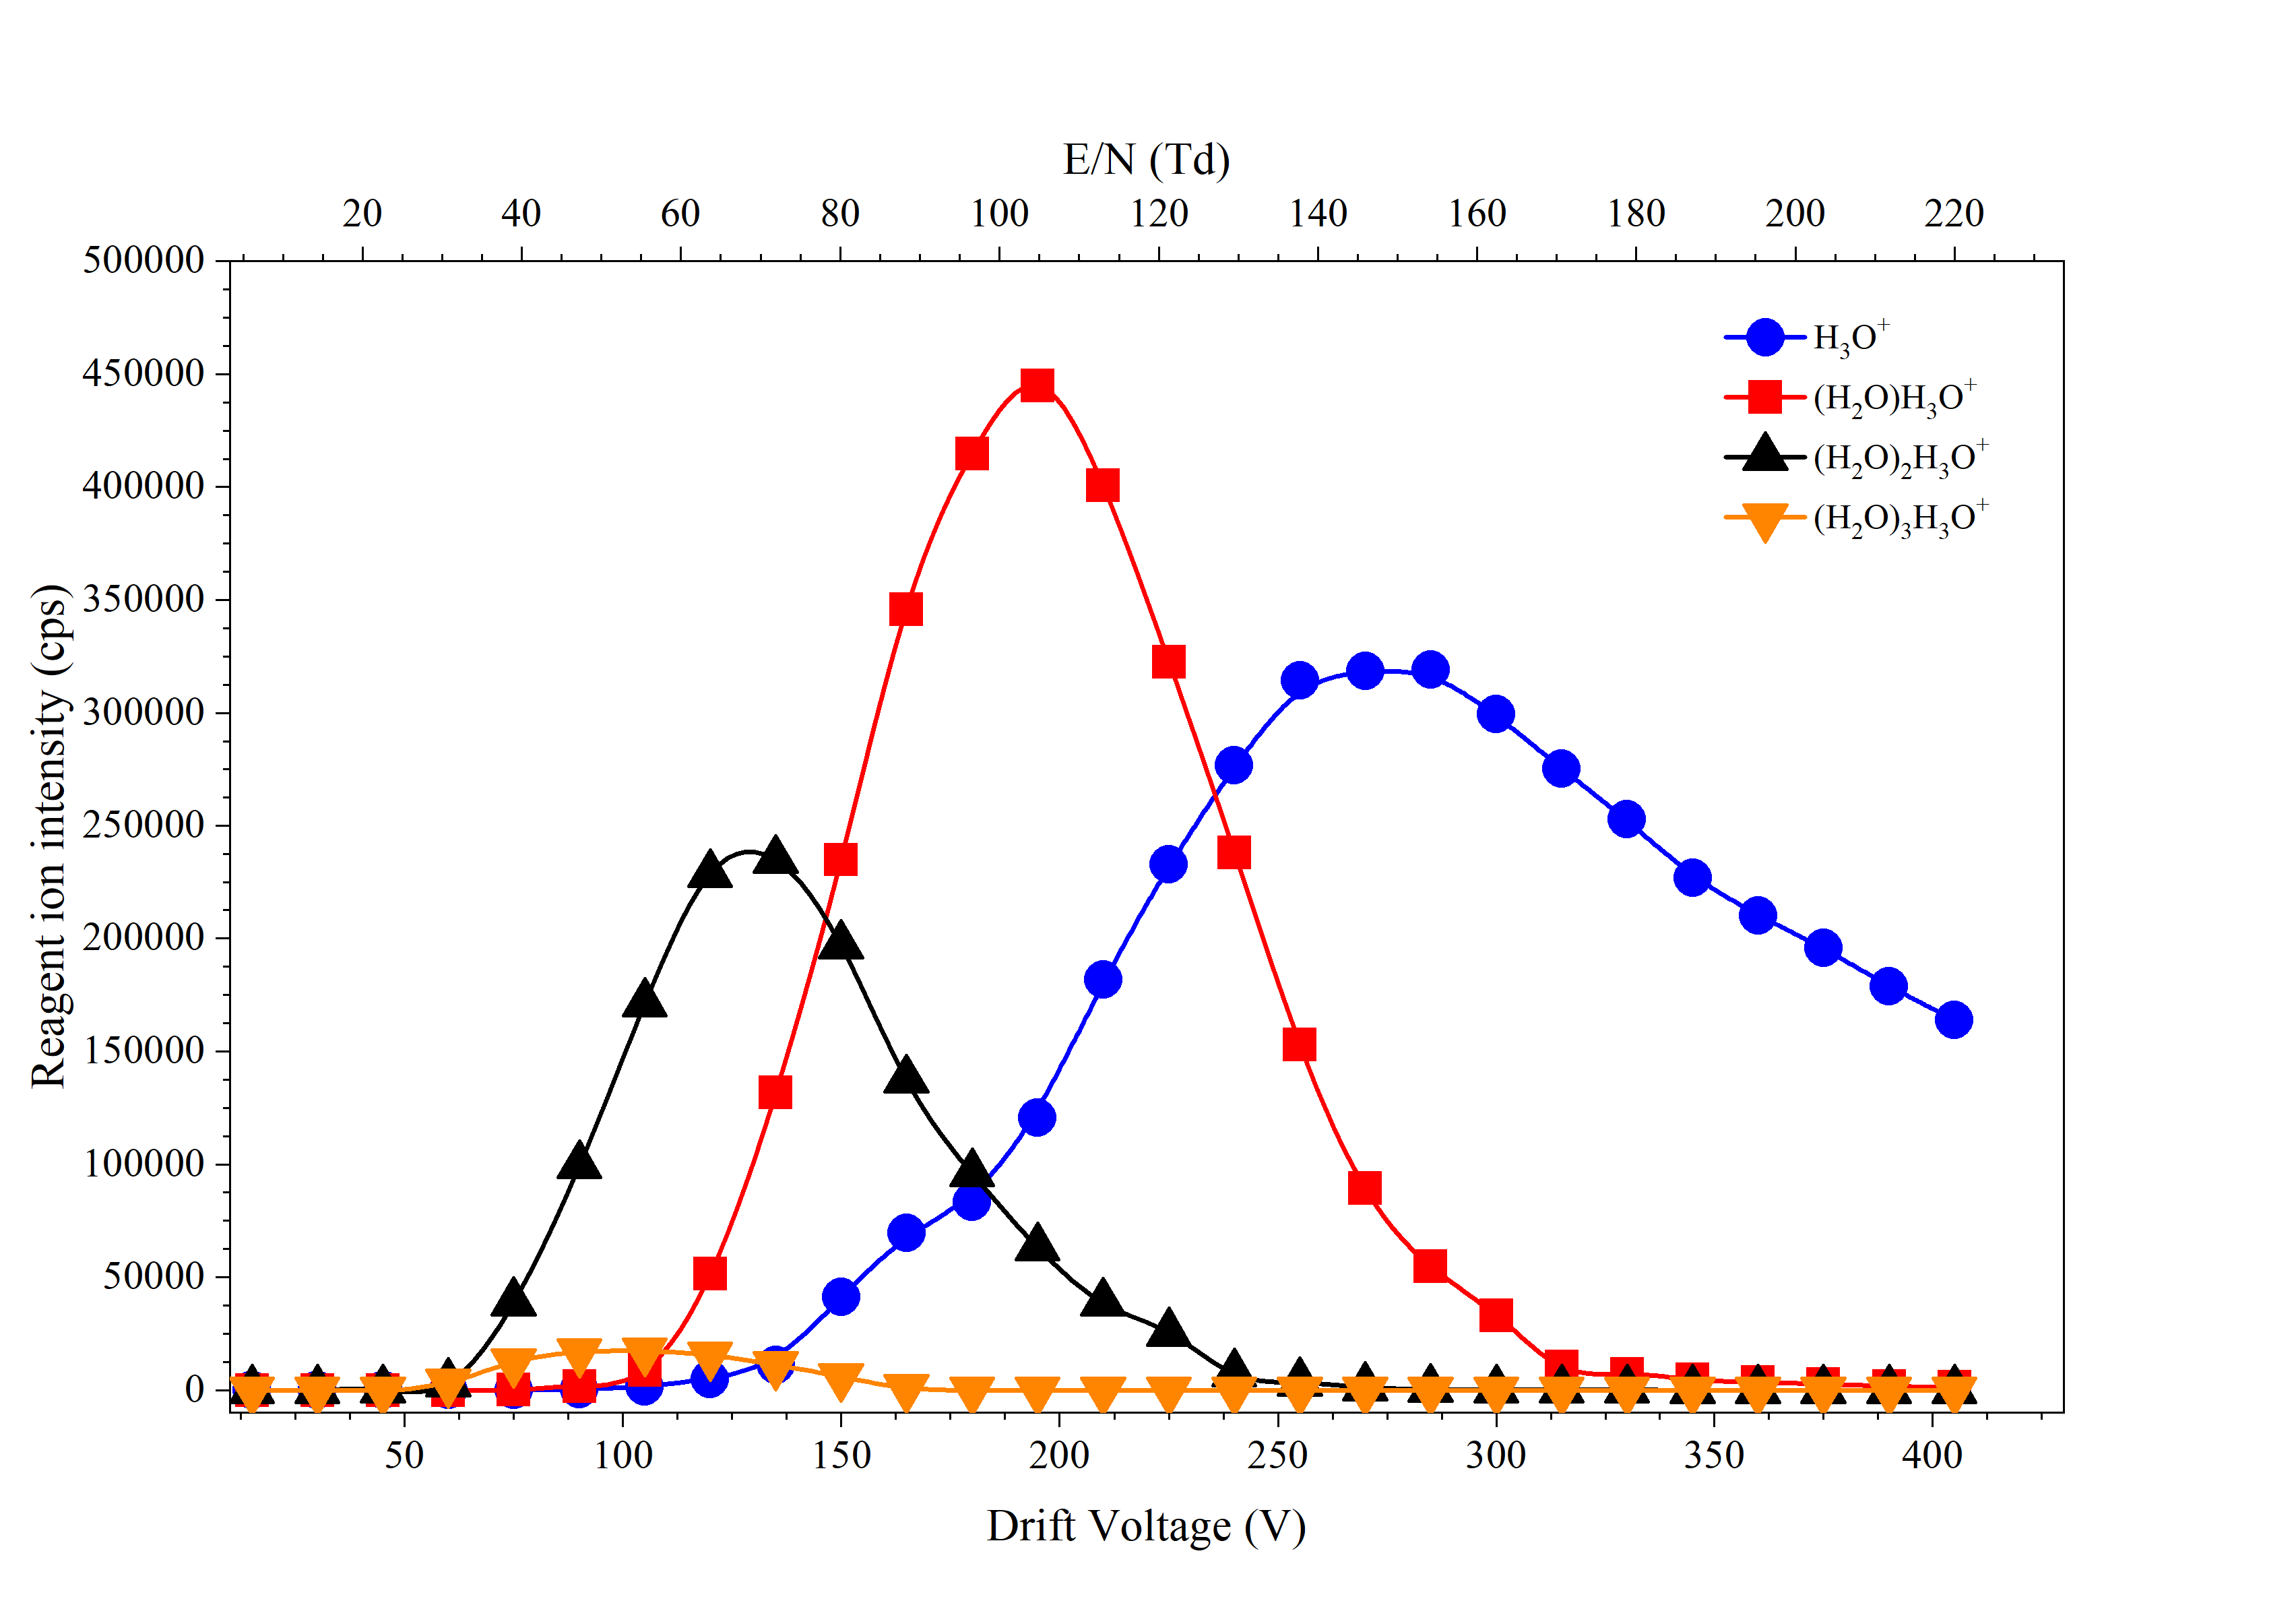
\includegraphics[width=0.48\linewidth]{pics/DPM_clusters_littoral.png}
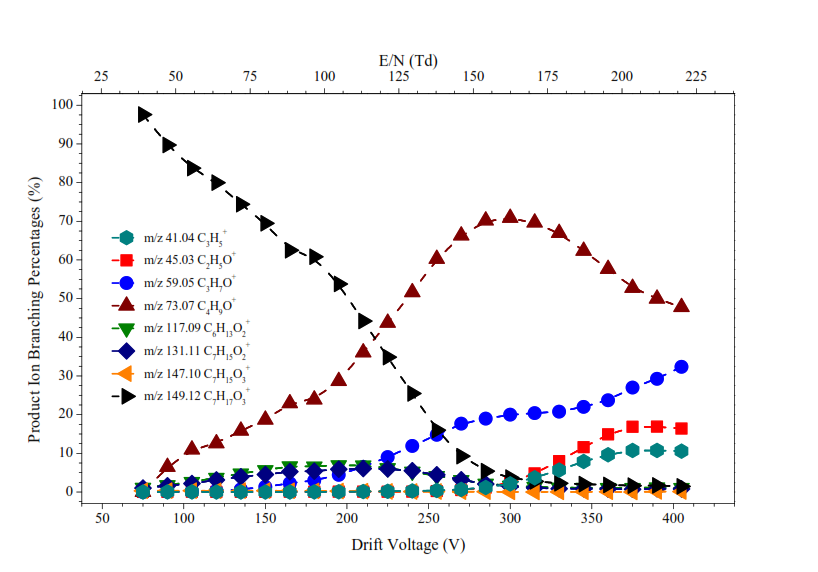
\includegraphics[width=0.48\linewidth]{pics/DPM_BR_lit.png}}
\vfill
\sidesubfloat[]{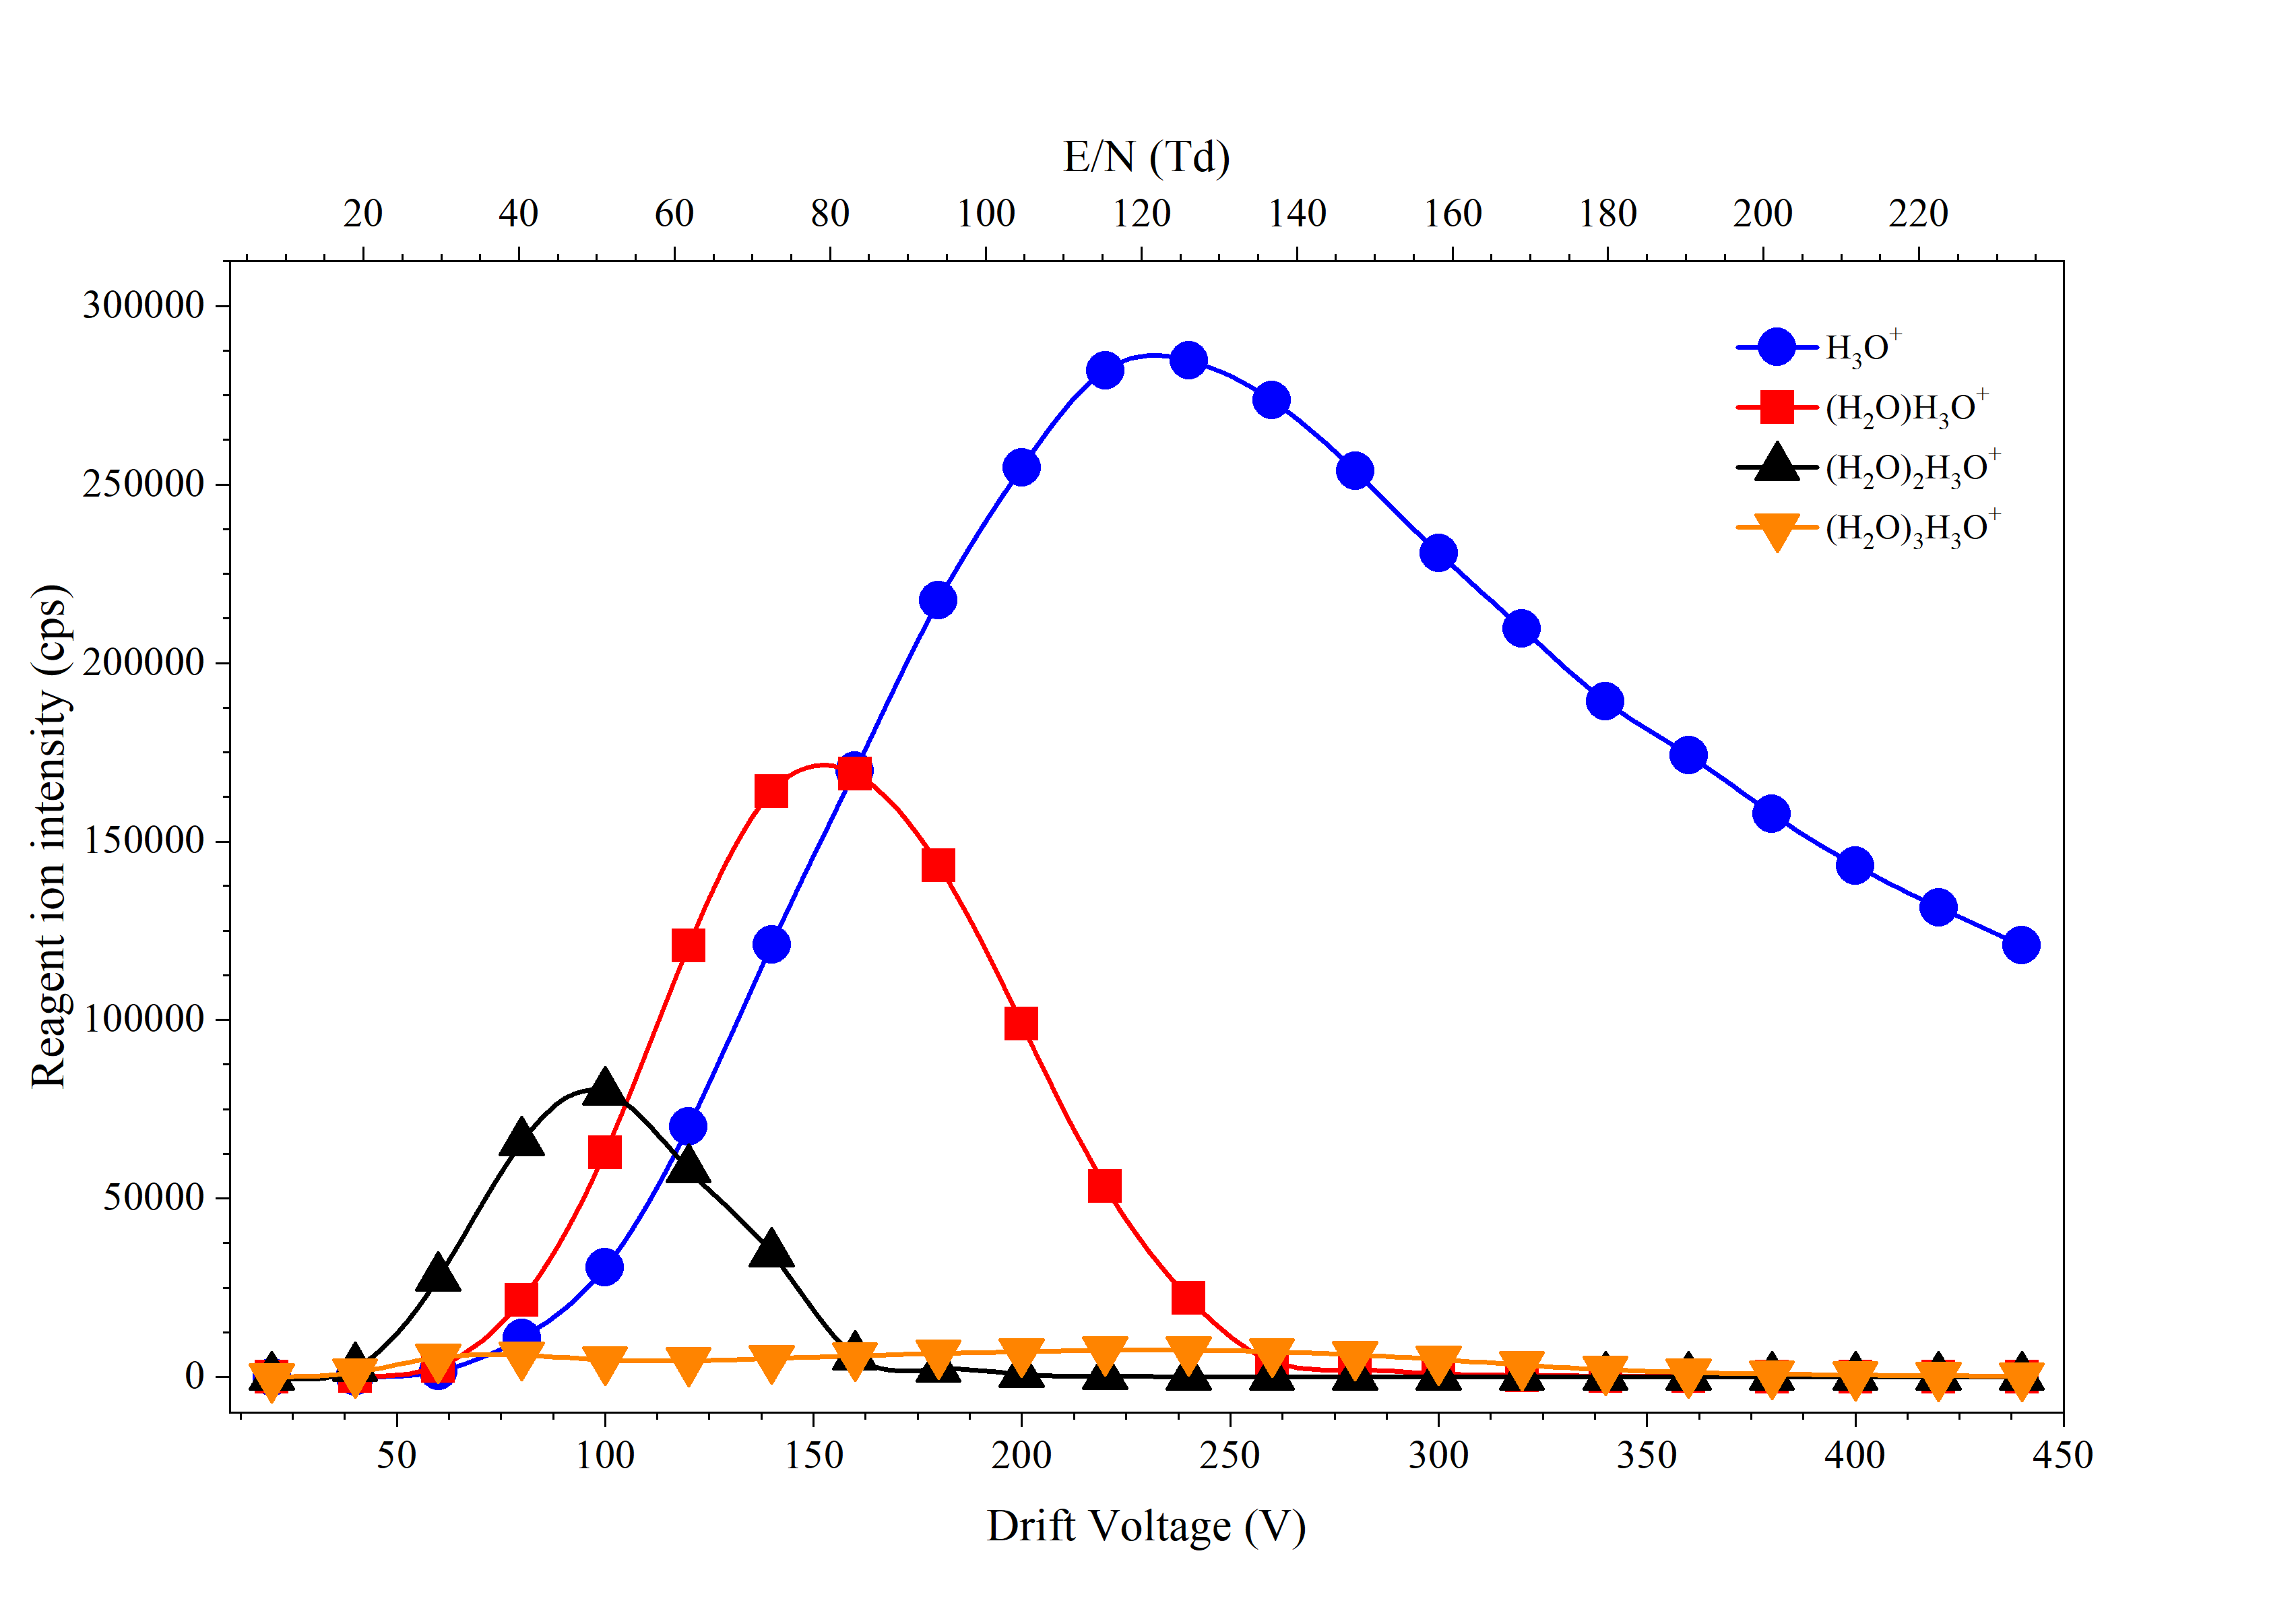
\includegraphics[width=0.48\linewidth]{pics/DPM_clusters_lynx_humid.png}
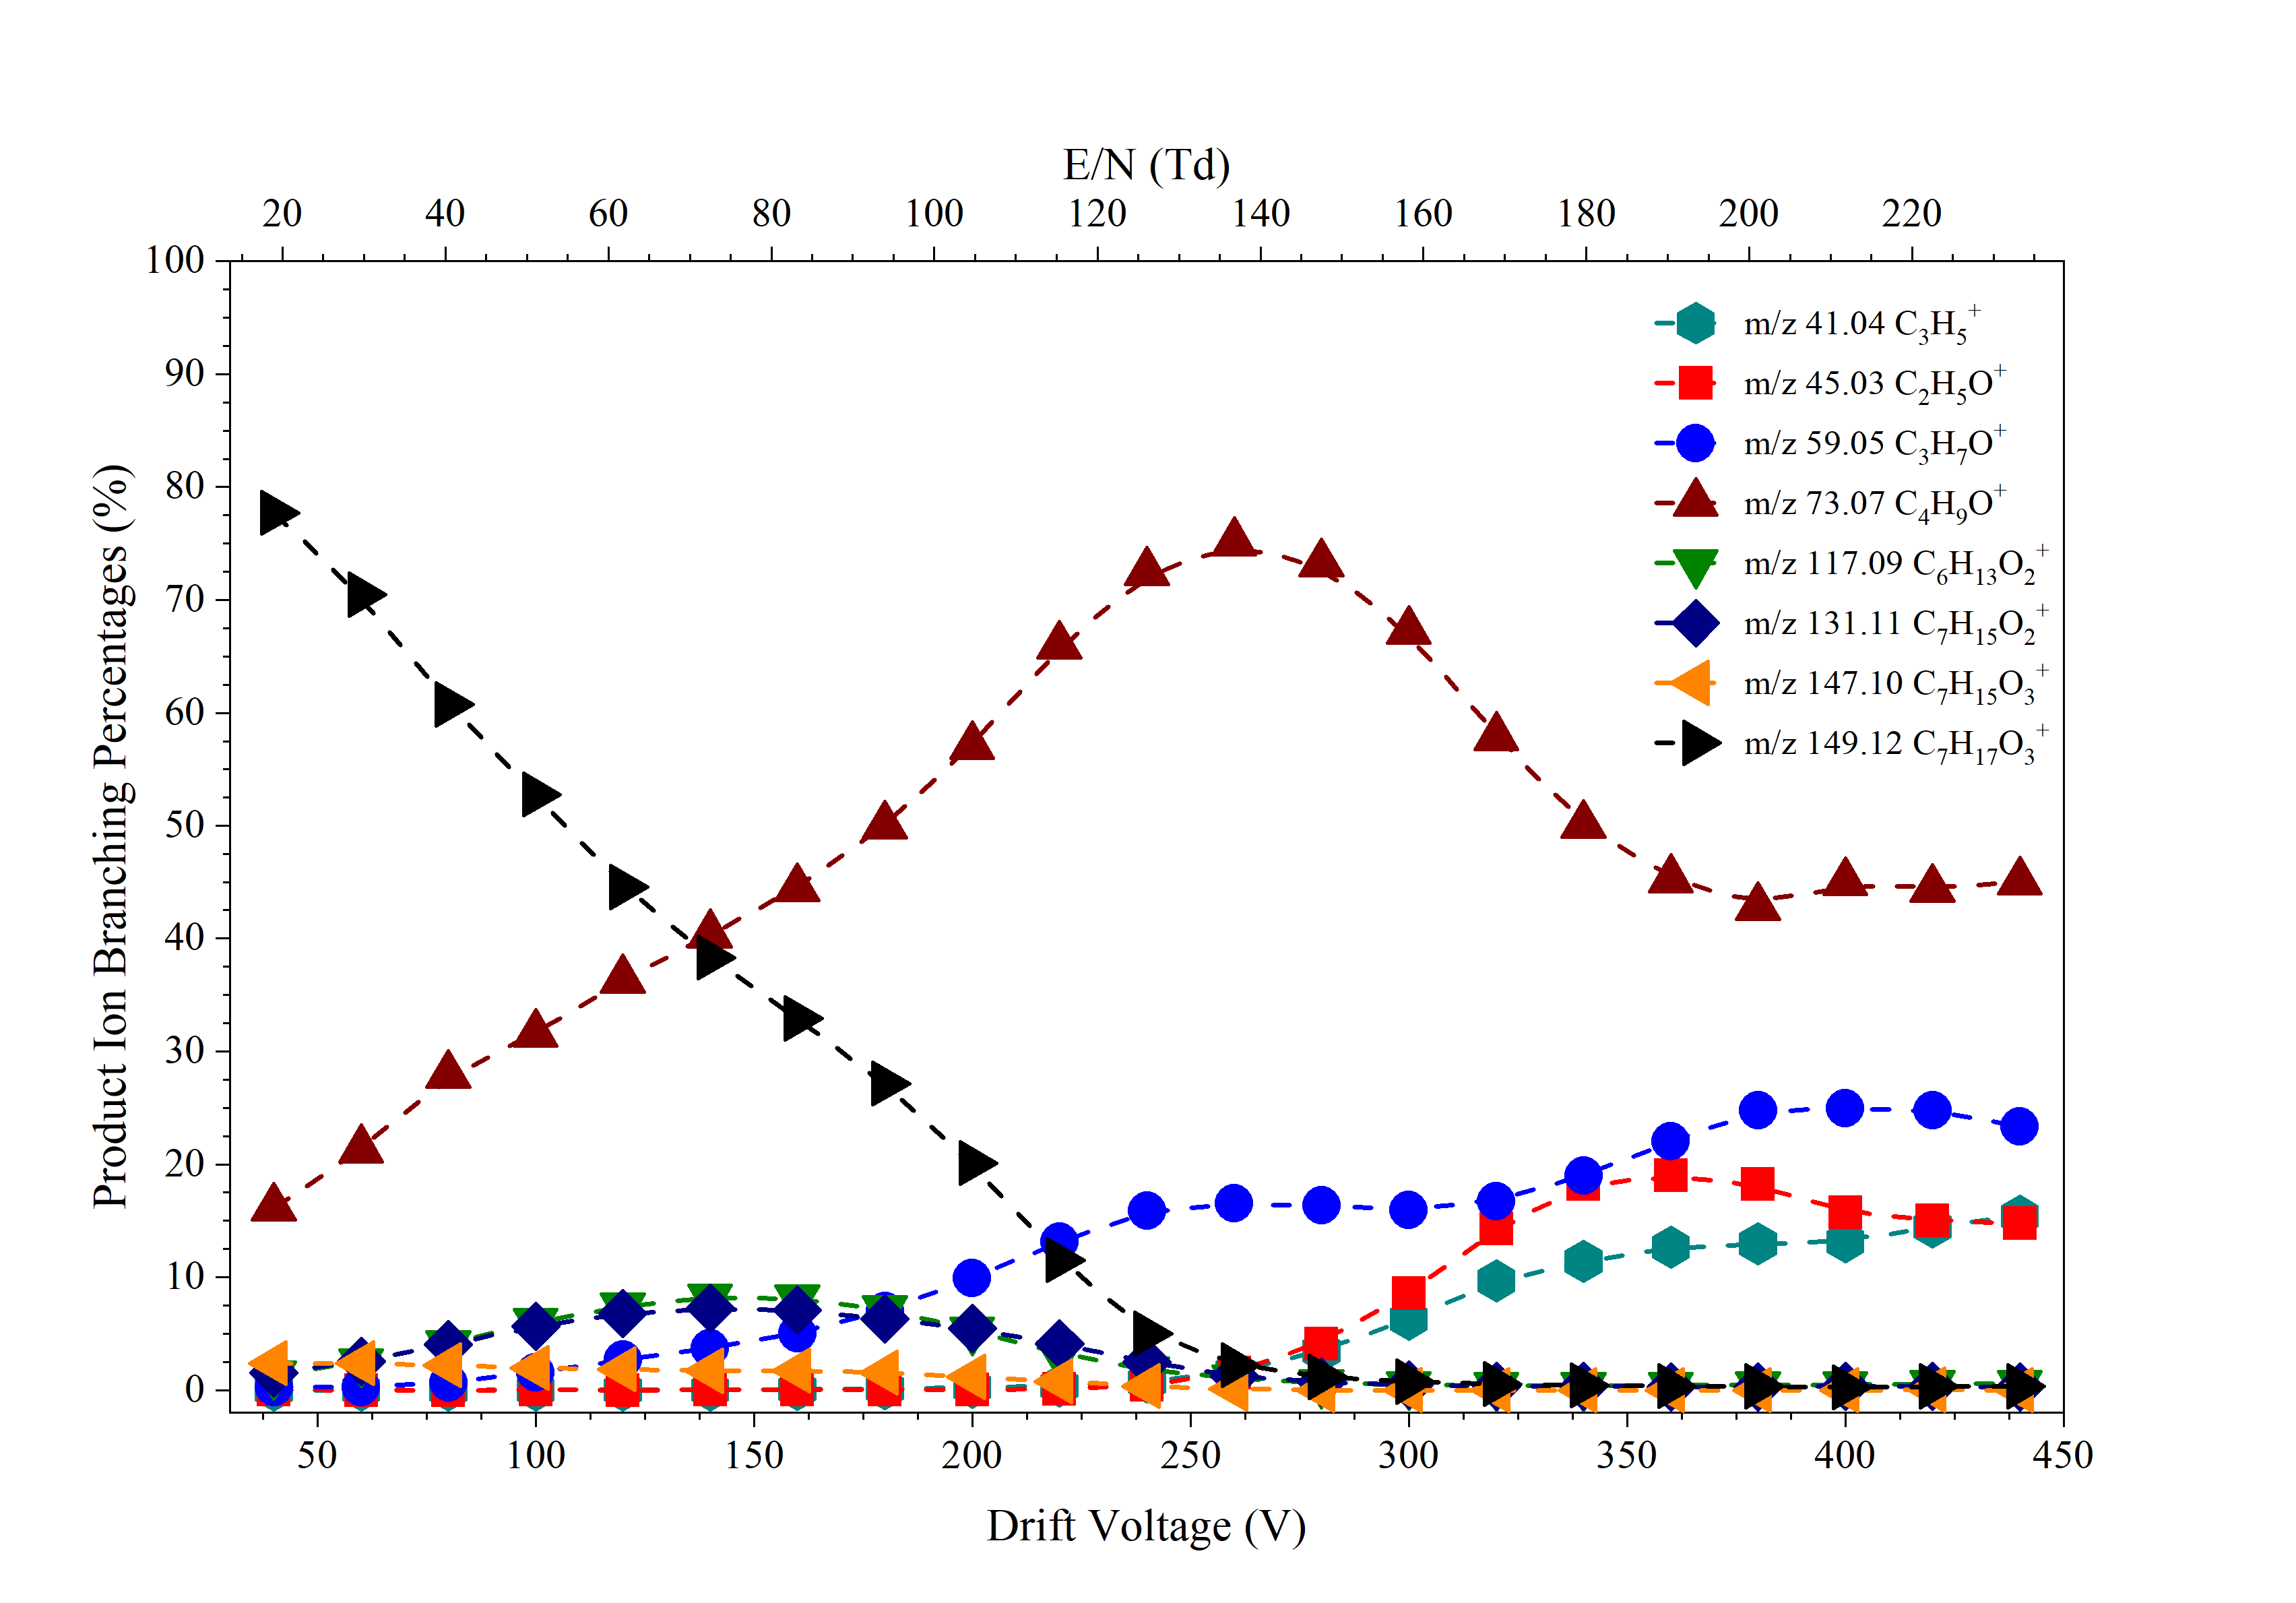
\includegraphics[width=0.48\linewidth]{pics/DPM_humid_DC_lynx.png}}
\vfill
\sidesubfloat[]{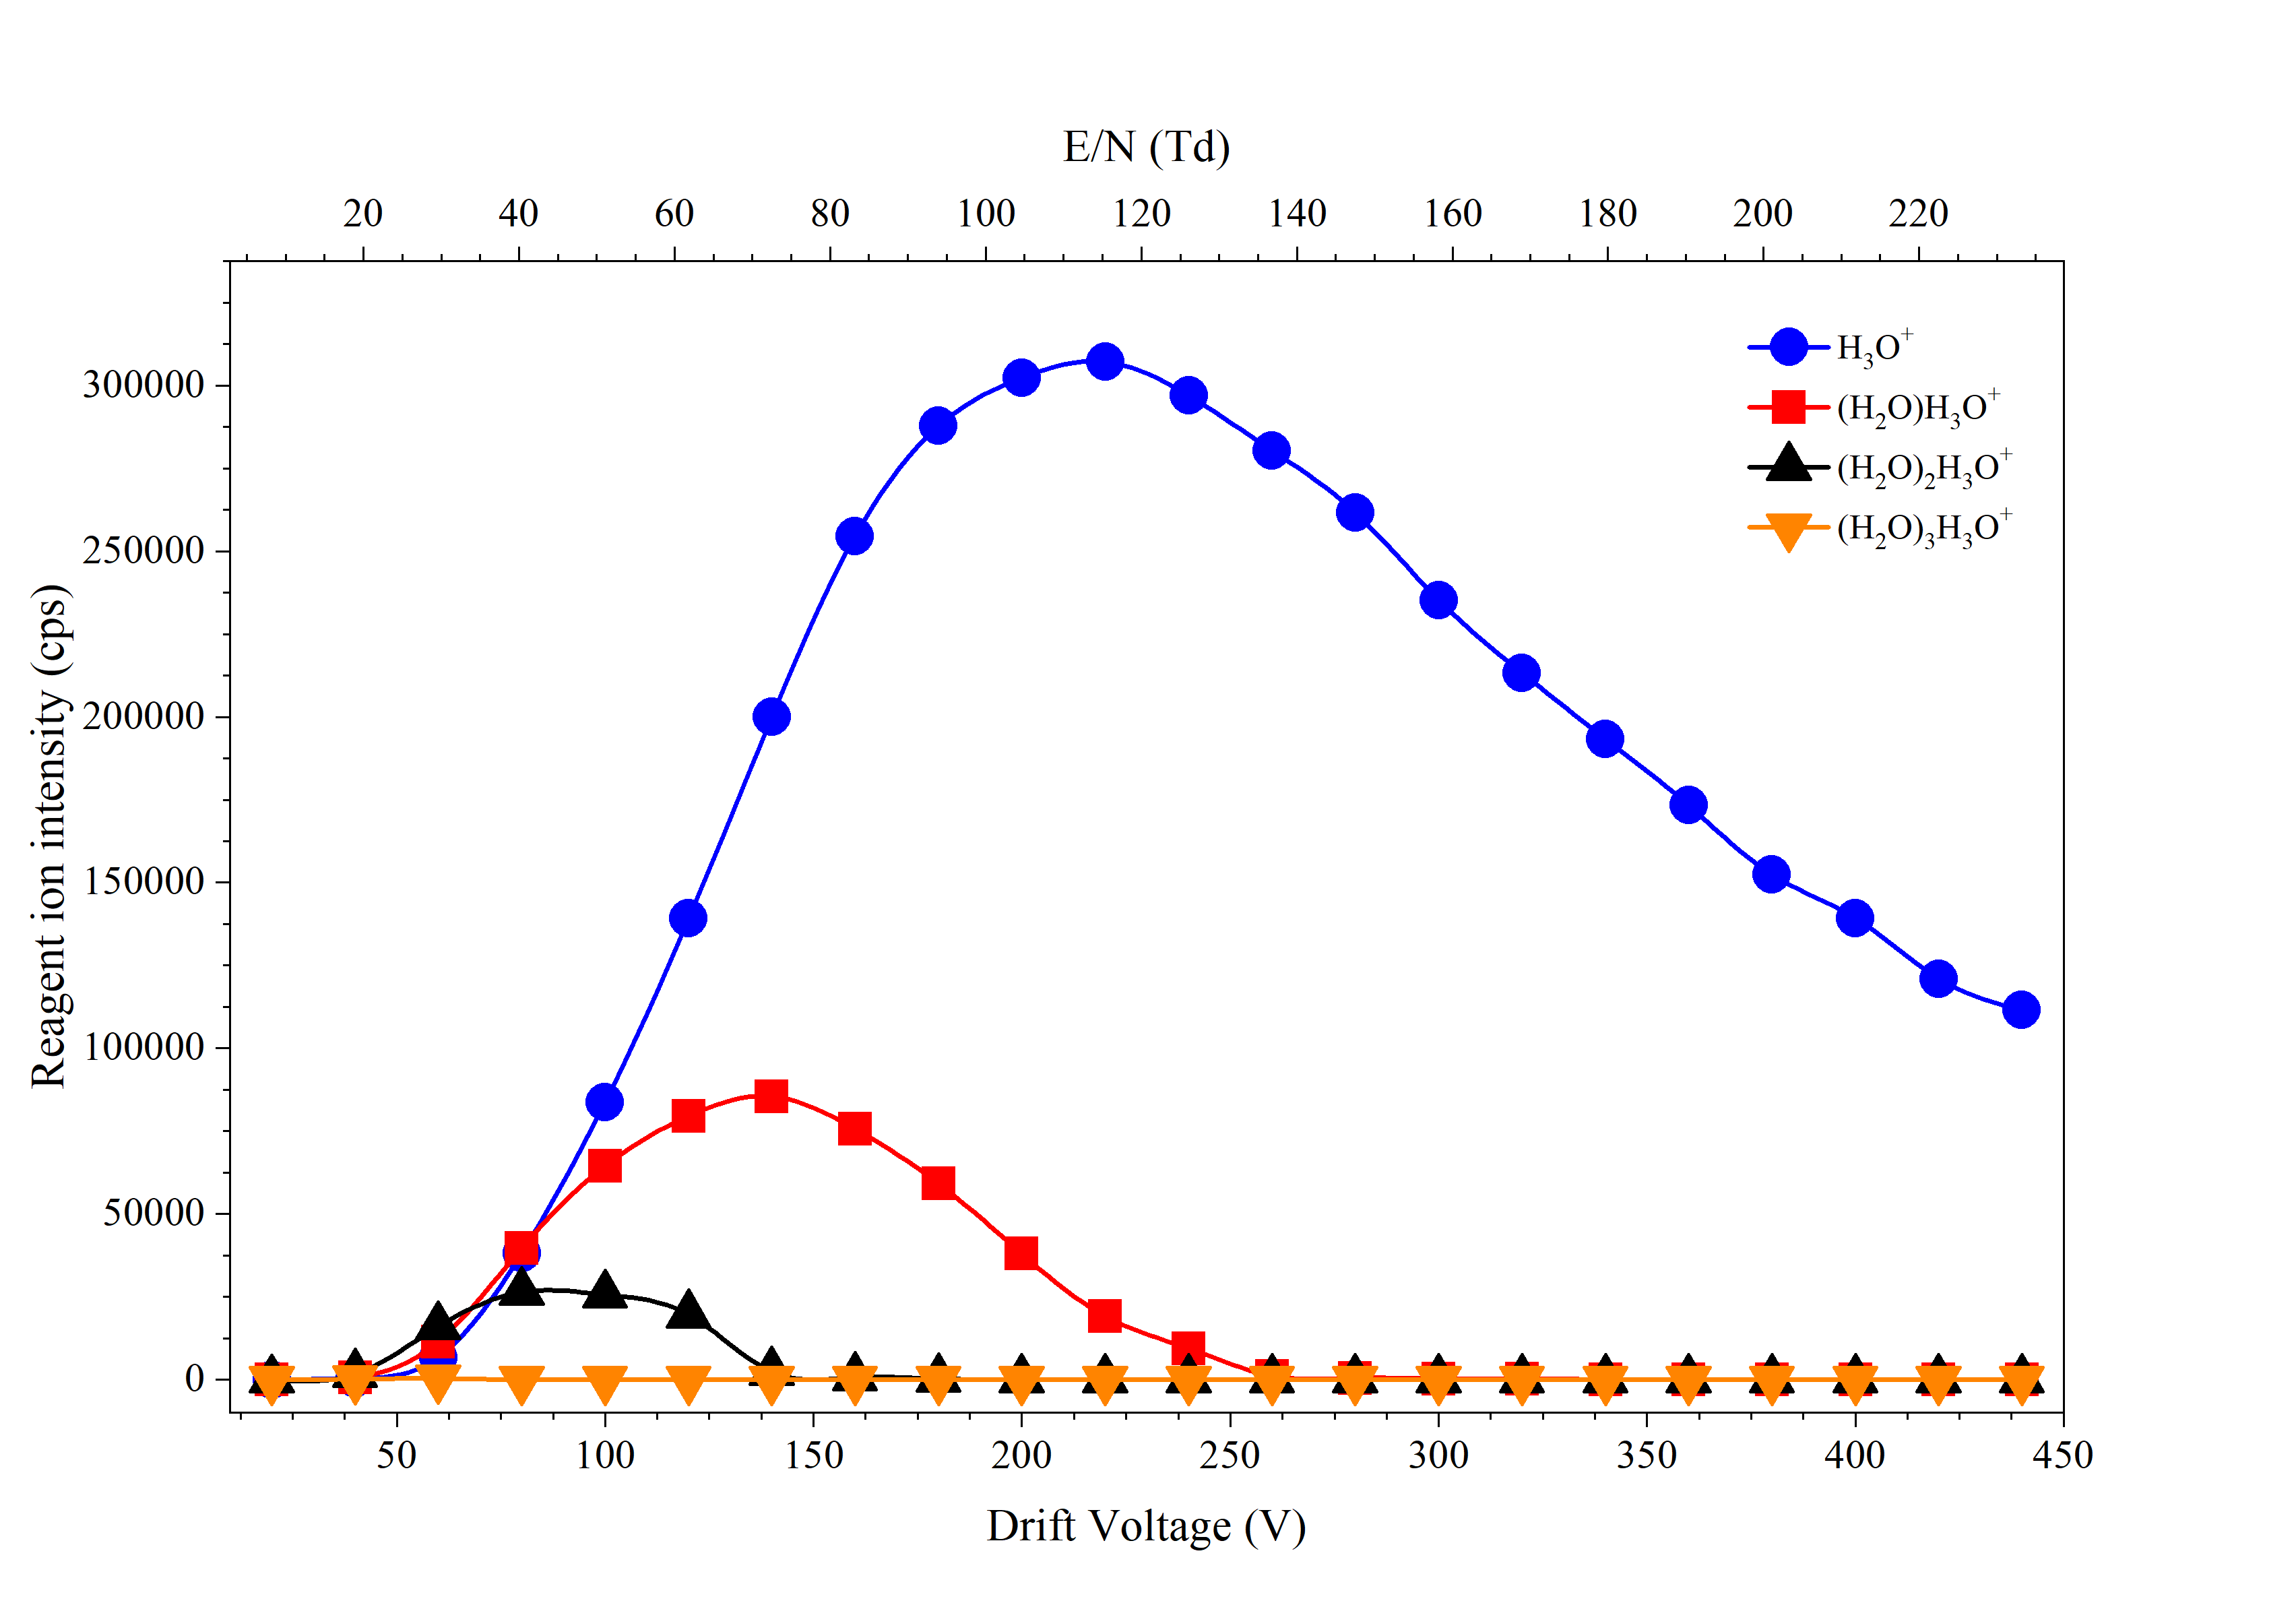
\includegraphics[width=0.48\linewidth]{pics/DPM_clusters_lynx_dry.png}
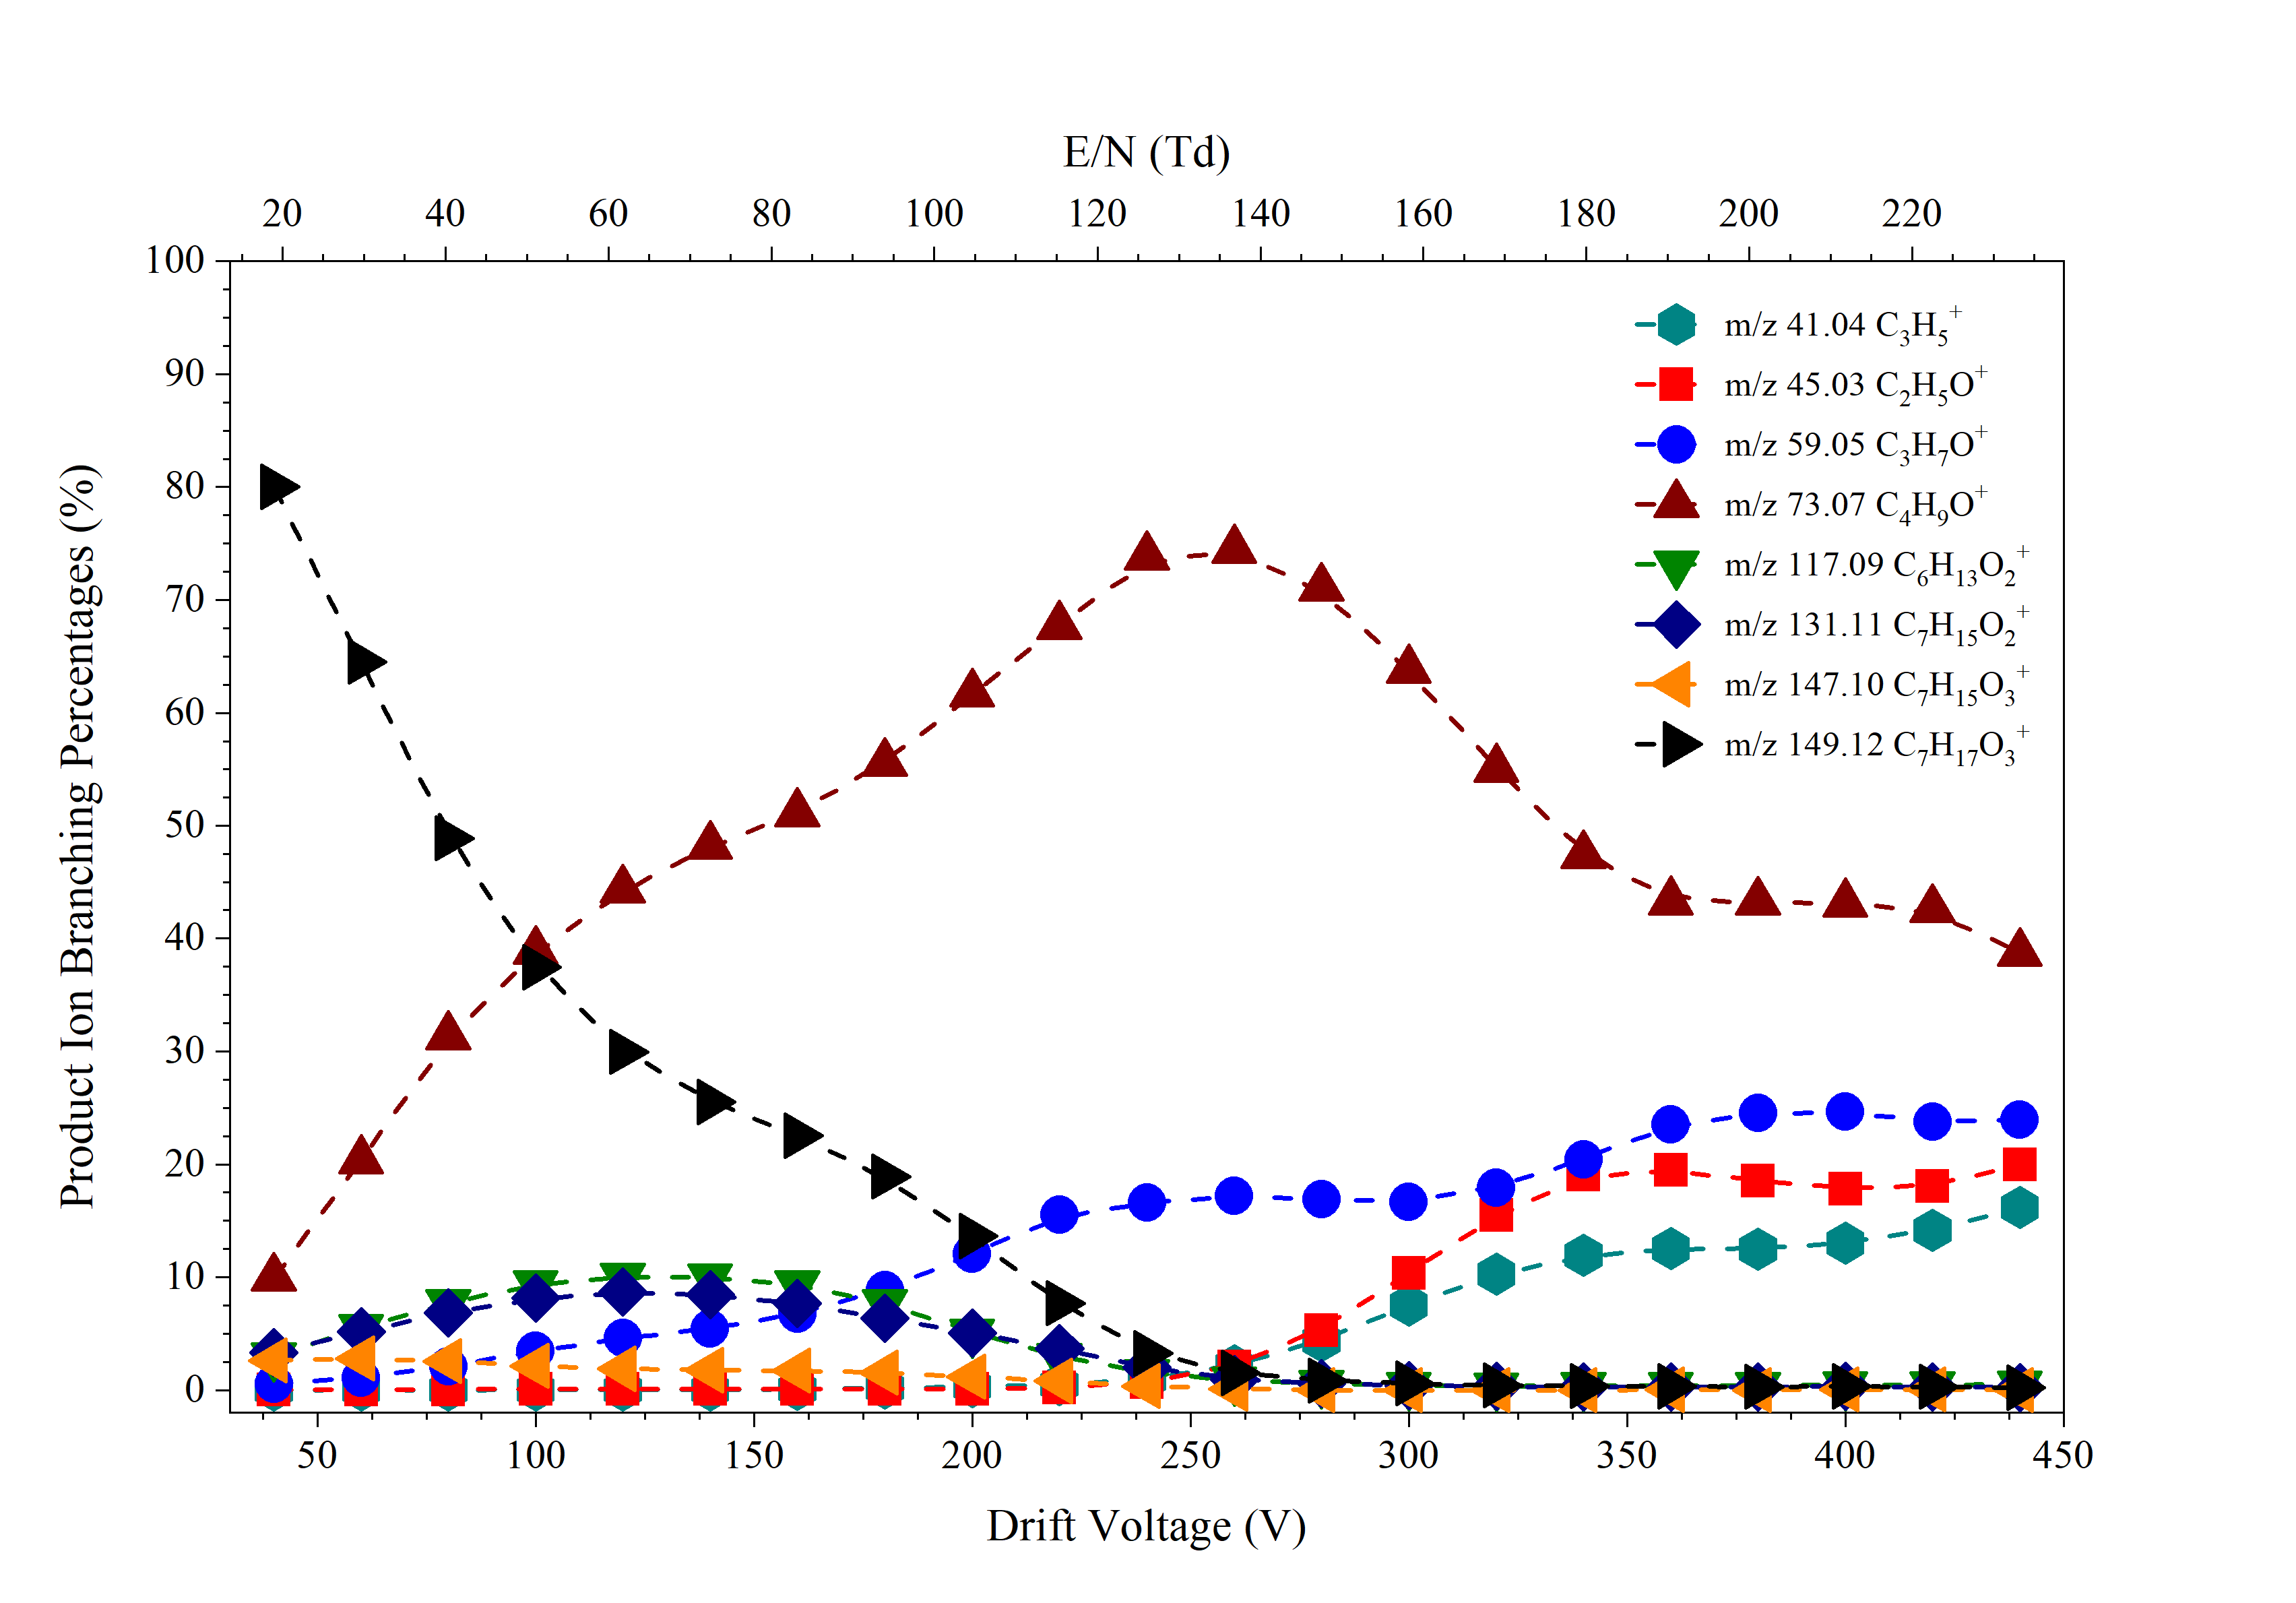
\includegraphics[width=0.48\linewidth]{pics/DPM_dry_DC_lynx.png}}
\vfill
\sidesubfloat[]{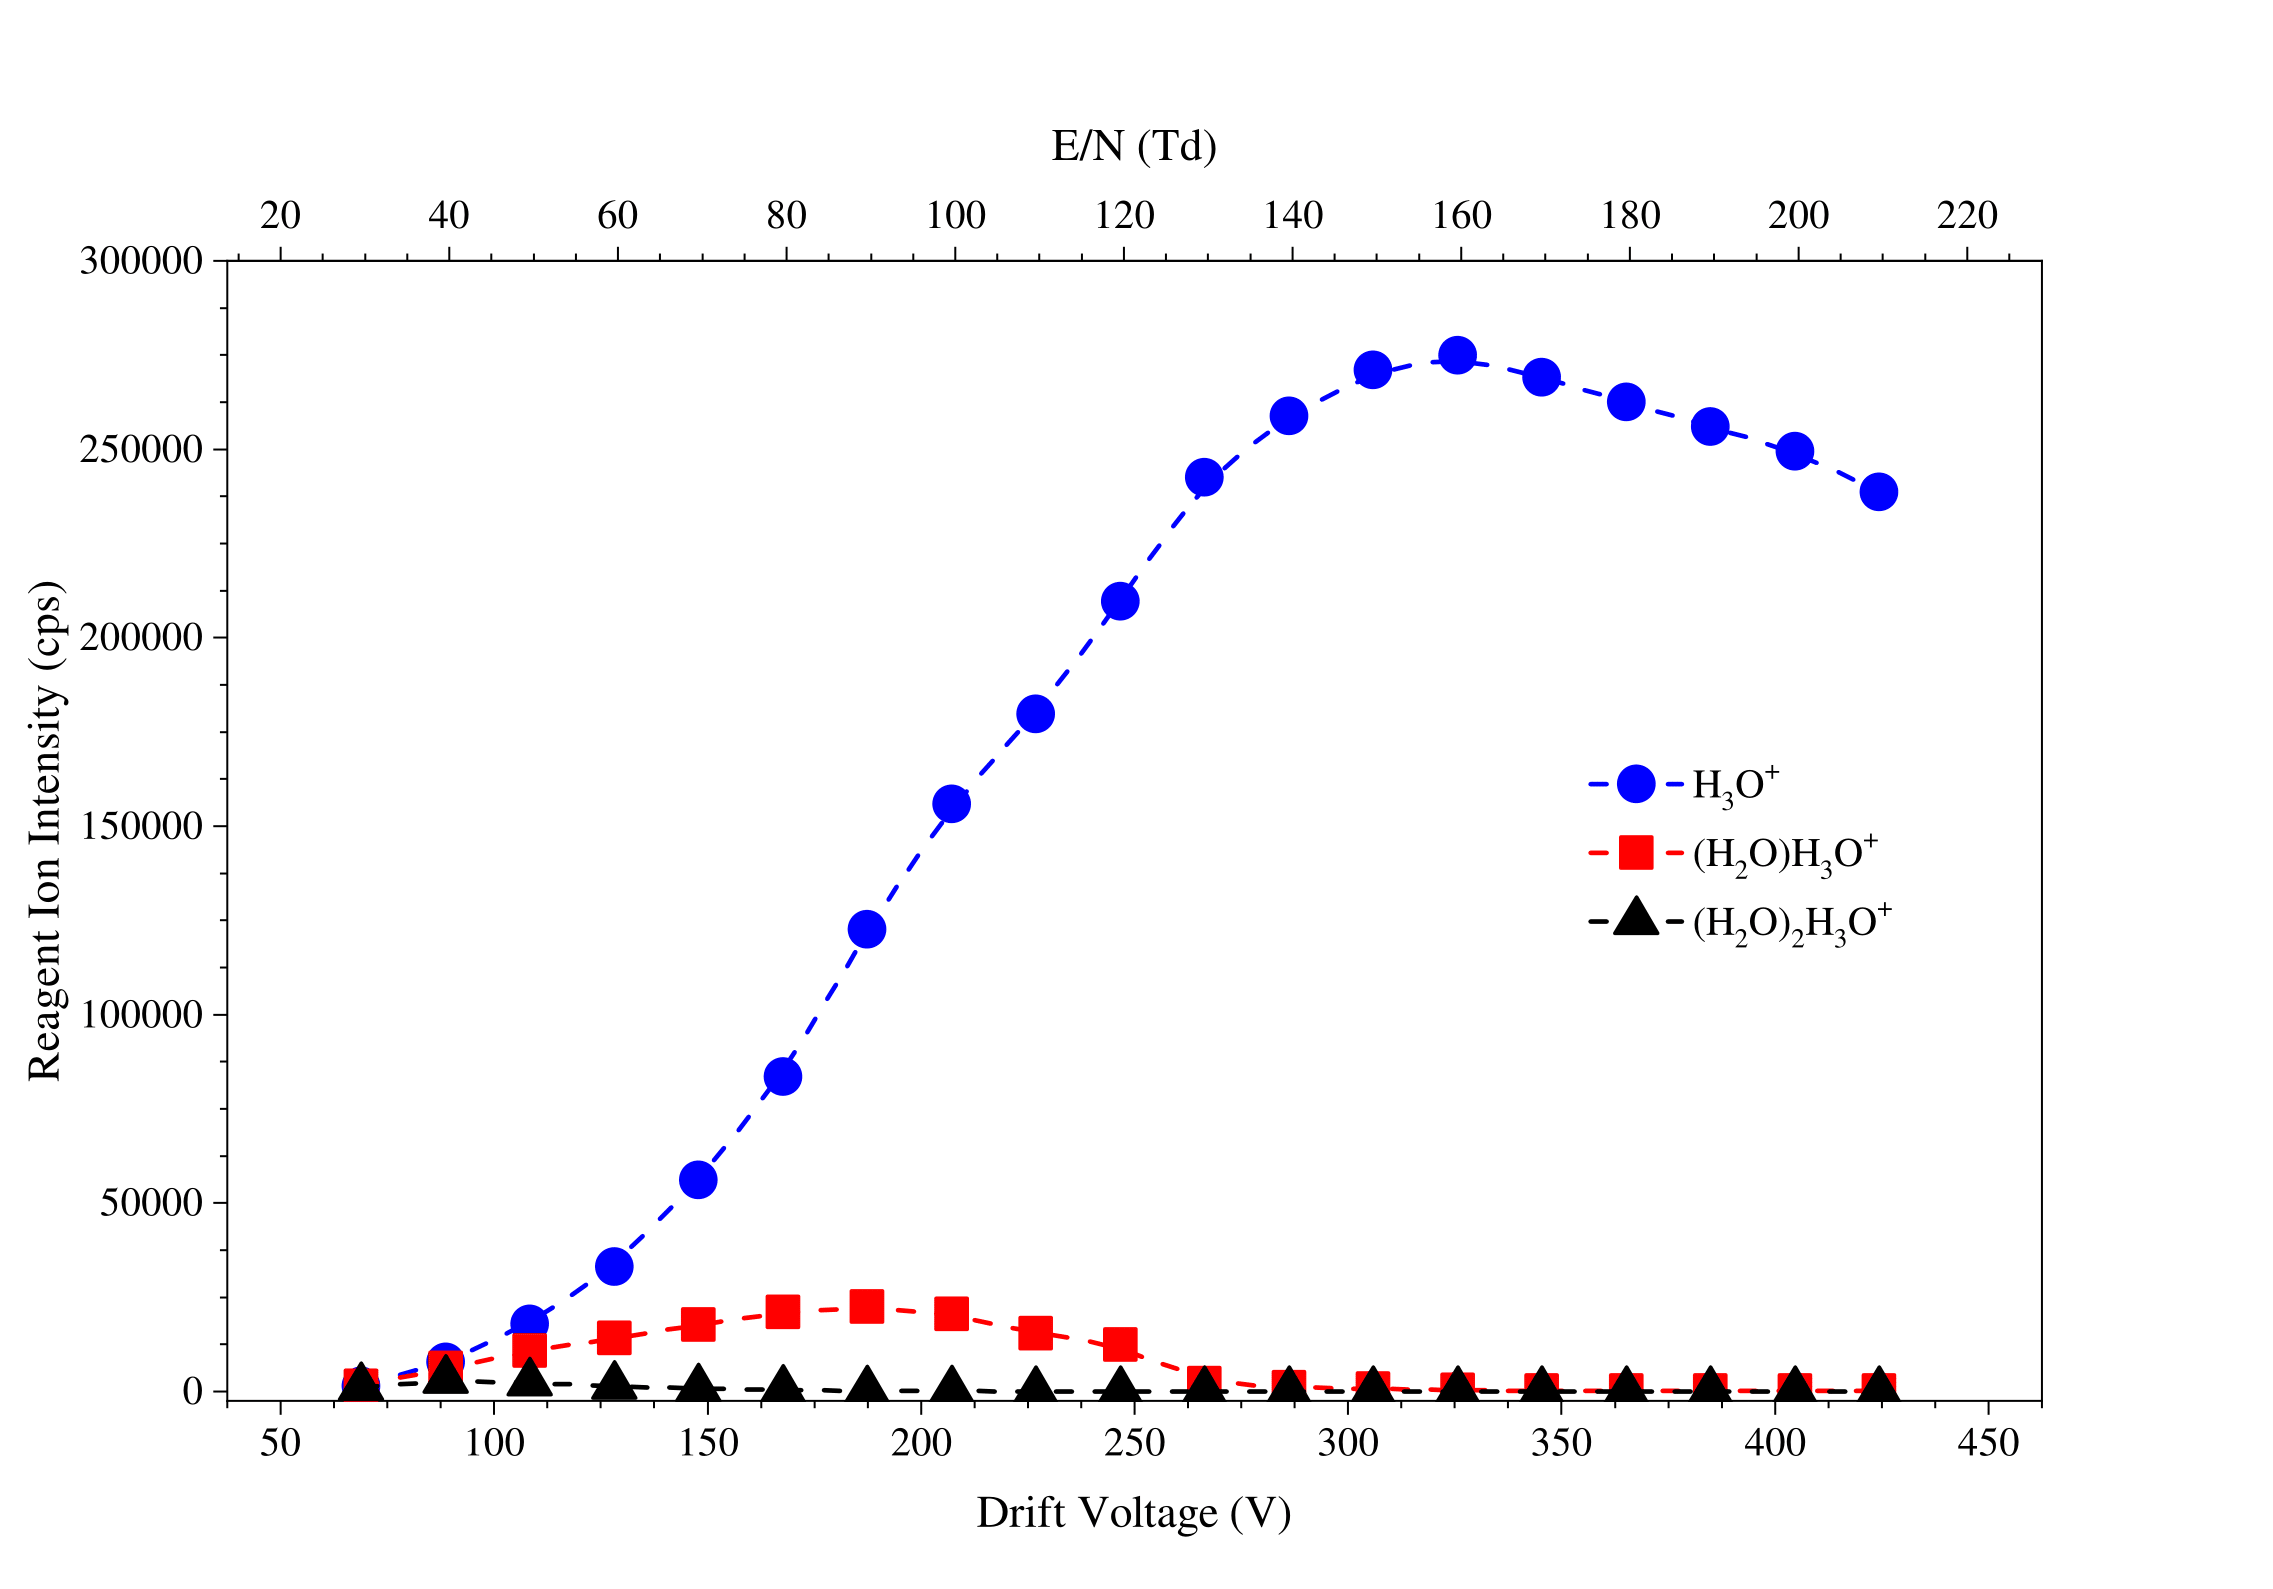
\includegraphics[width=0.48\linewidth]{pics/RIDPM-1.png}
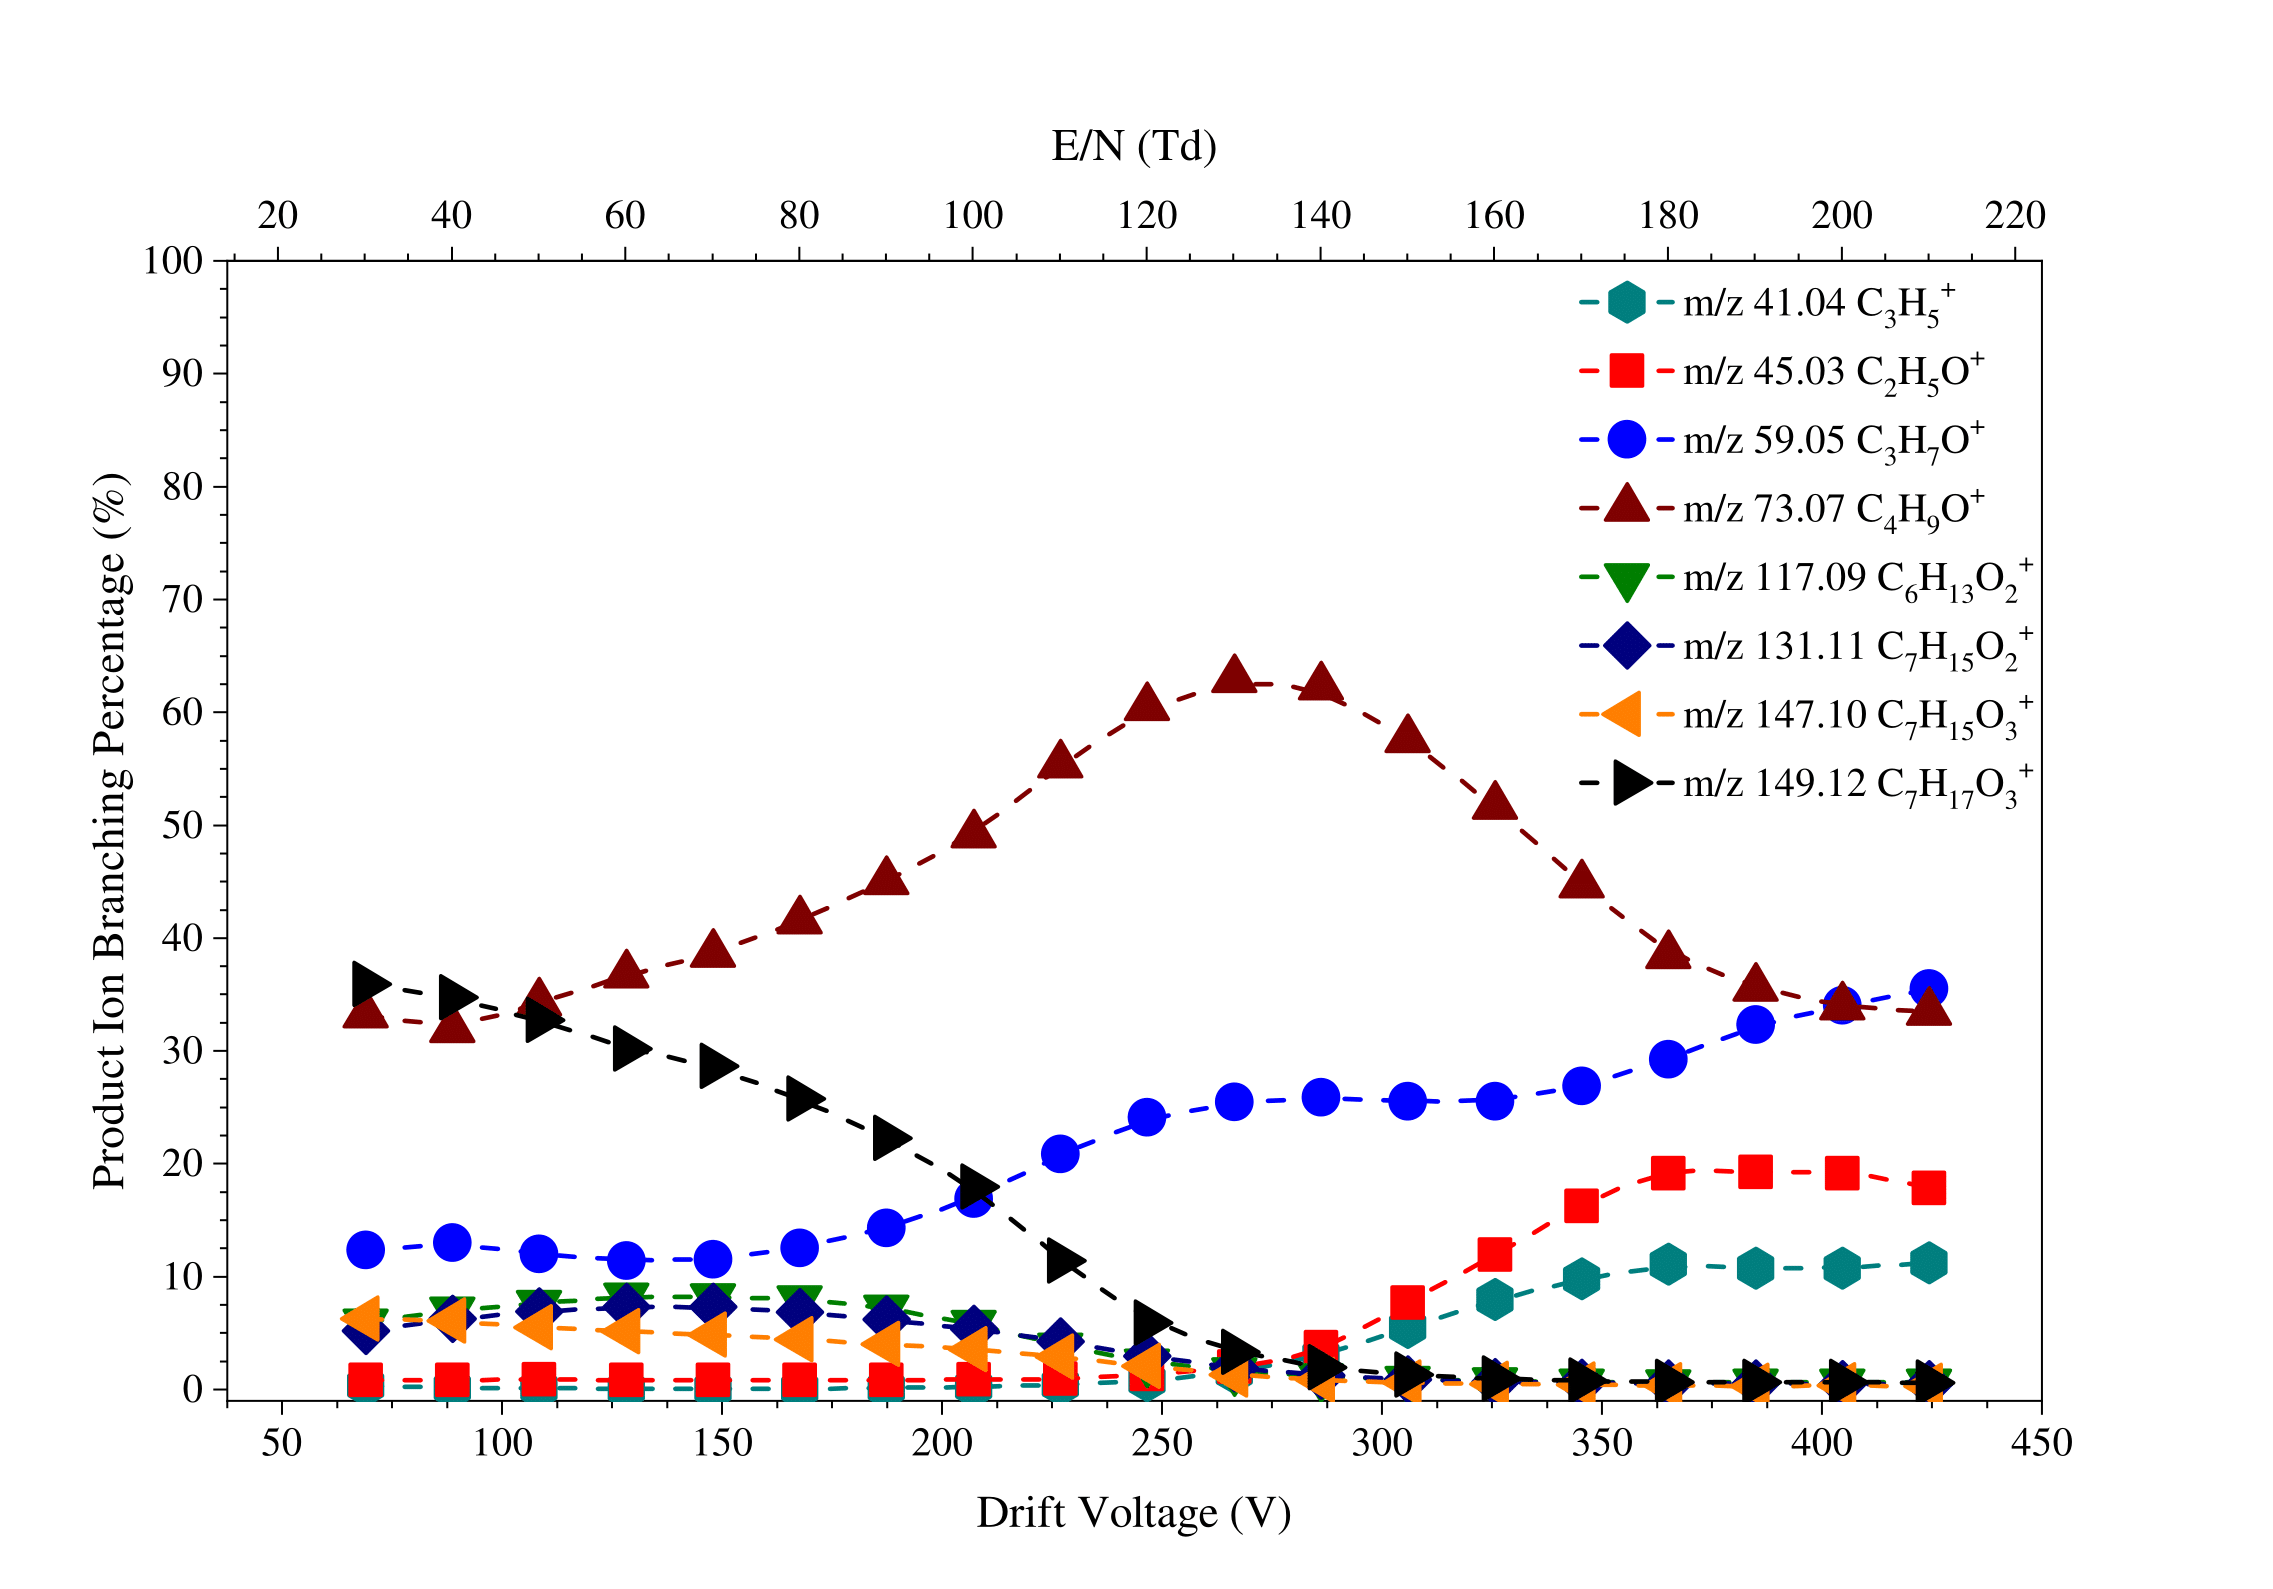
\includegraphics[width=0.48\linewidth]{pics/DPM-1.png}}
\caption{Reagent ions intensity and DPM product ion distribution plots from  humid  (a) to dry (d) conditions.}
\label{fig:dpm}
\end{figure}

\begin{figure}%[h]
\centering
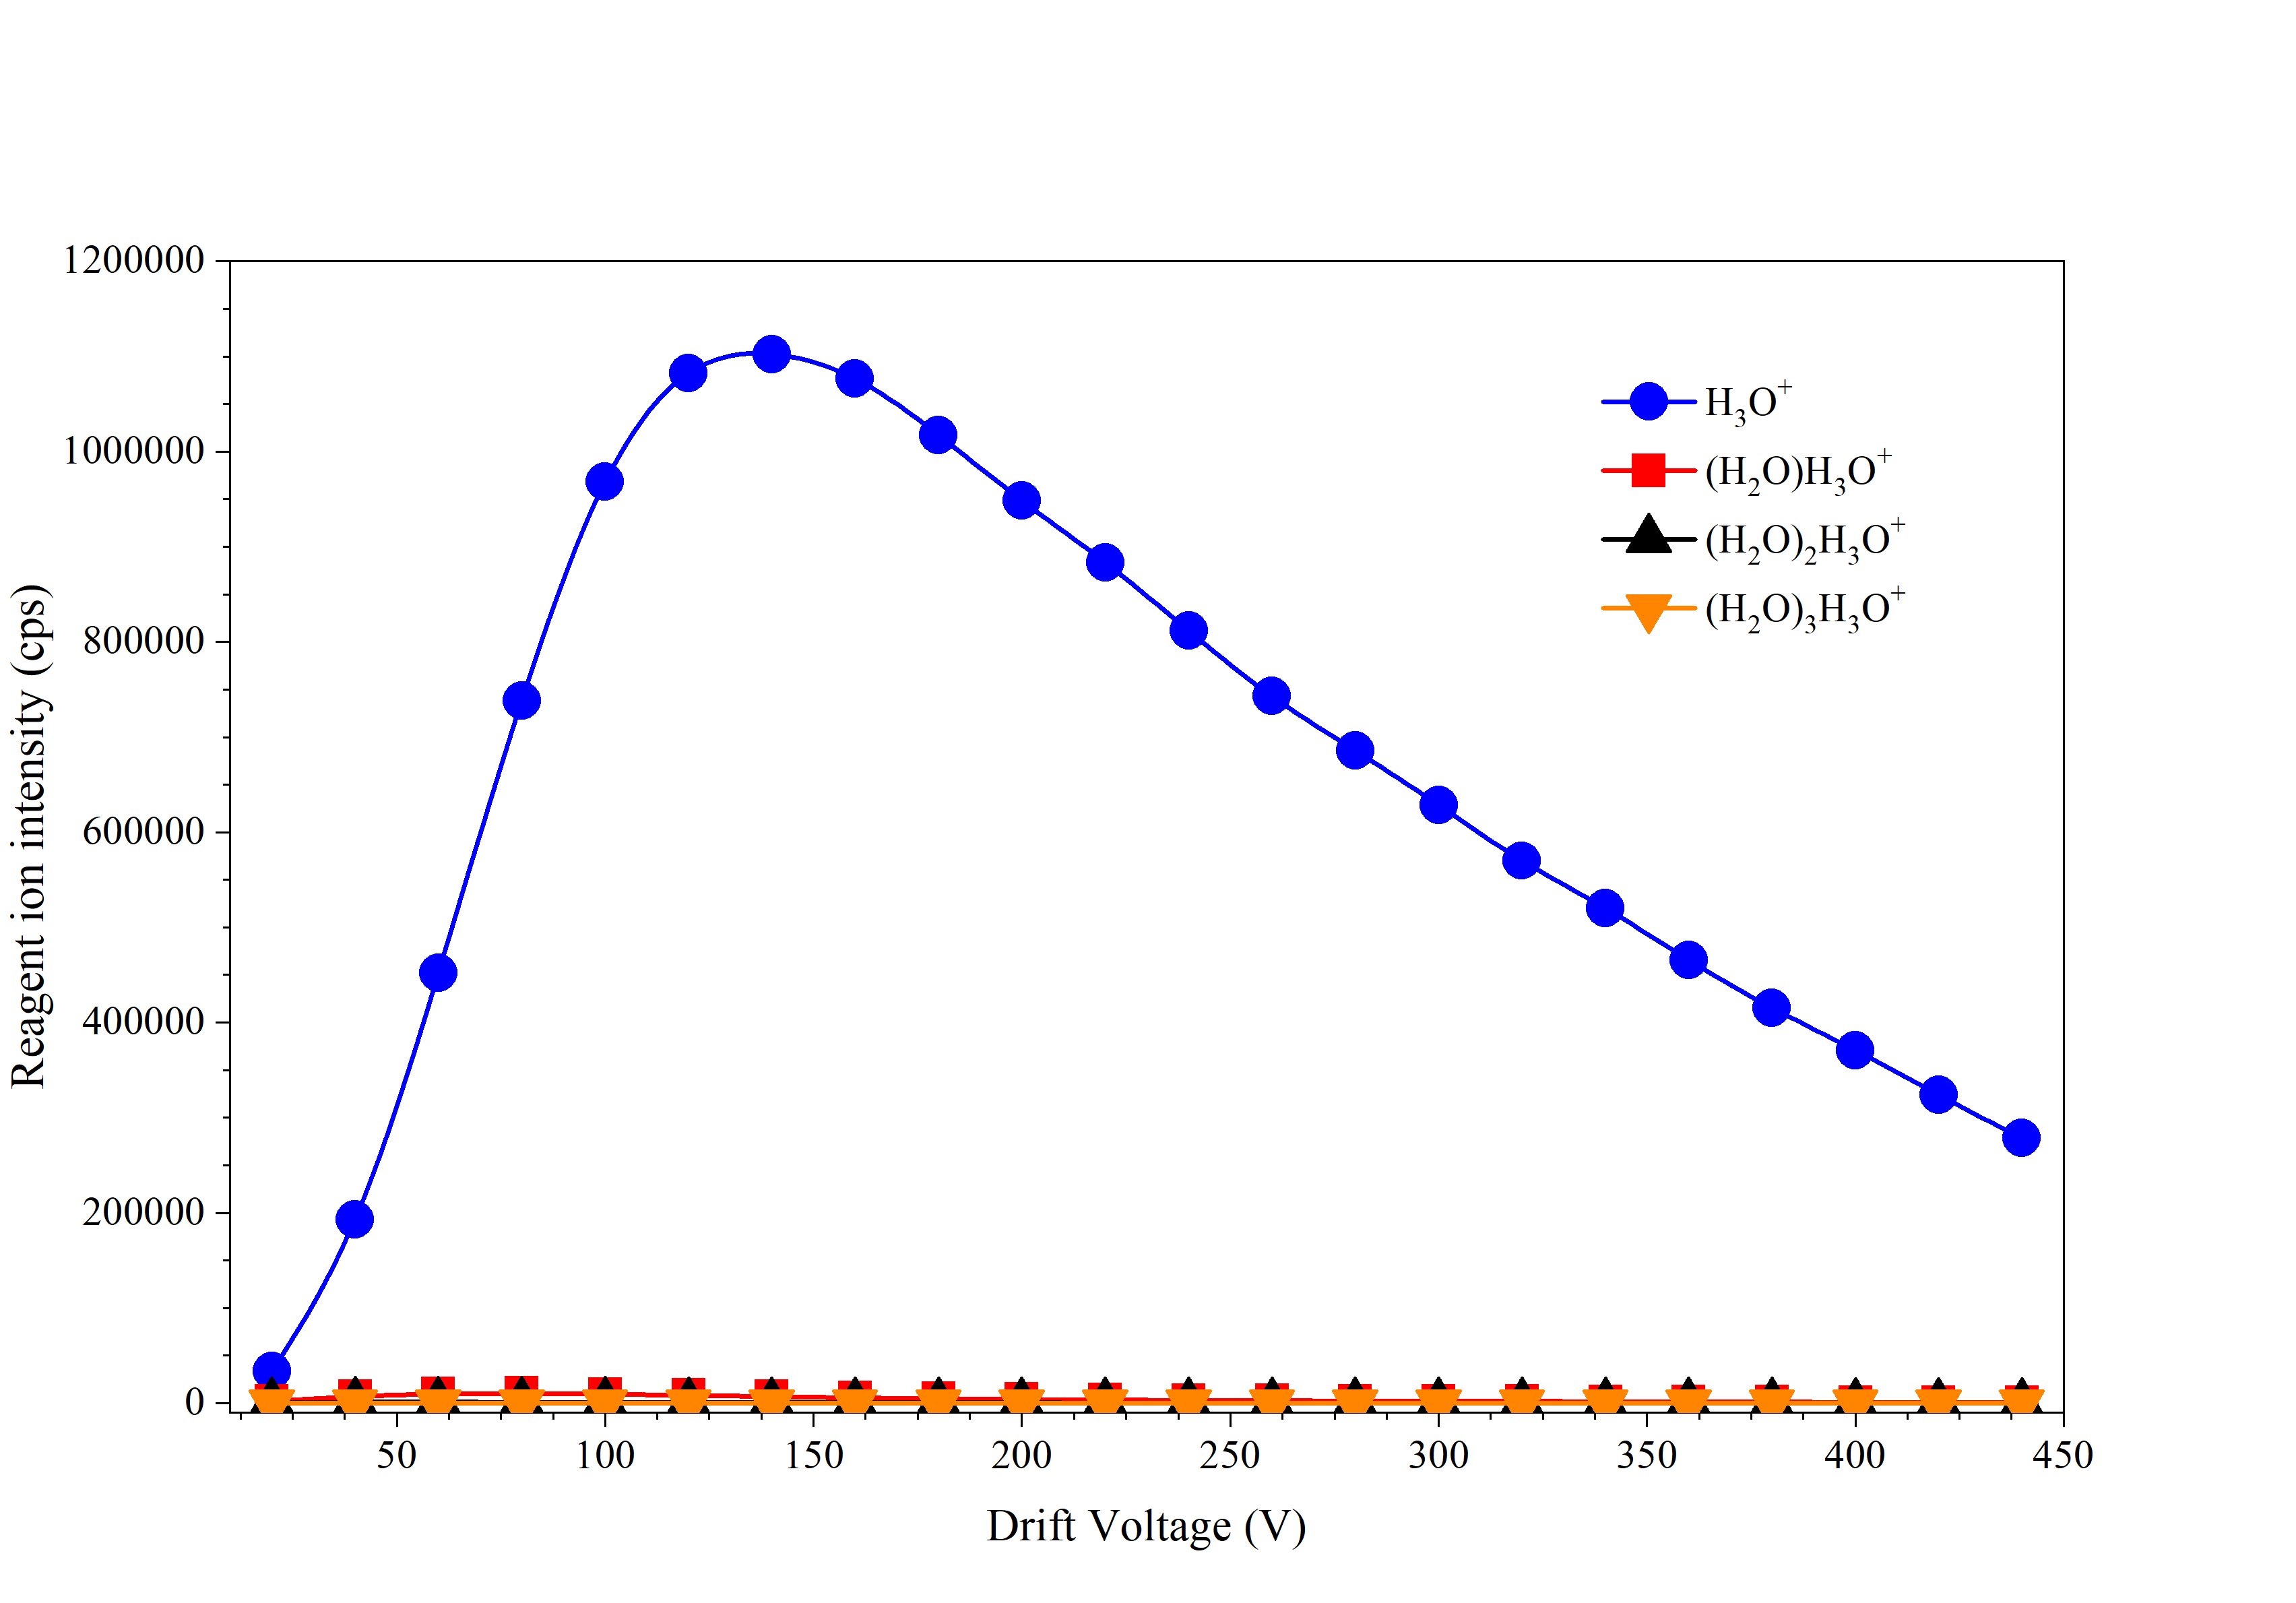
\includegraphics[width=0.48\linewidth]{pics/DPM_clusters_humid_RF.png}
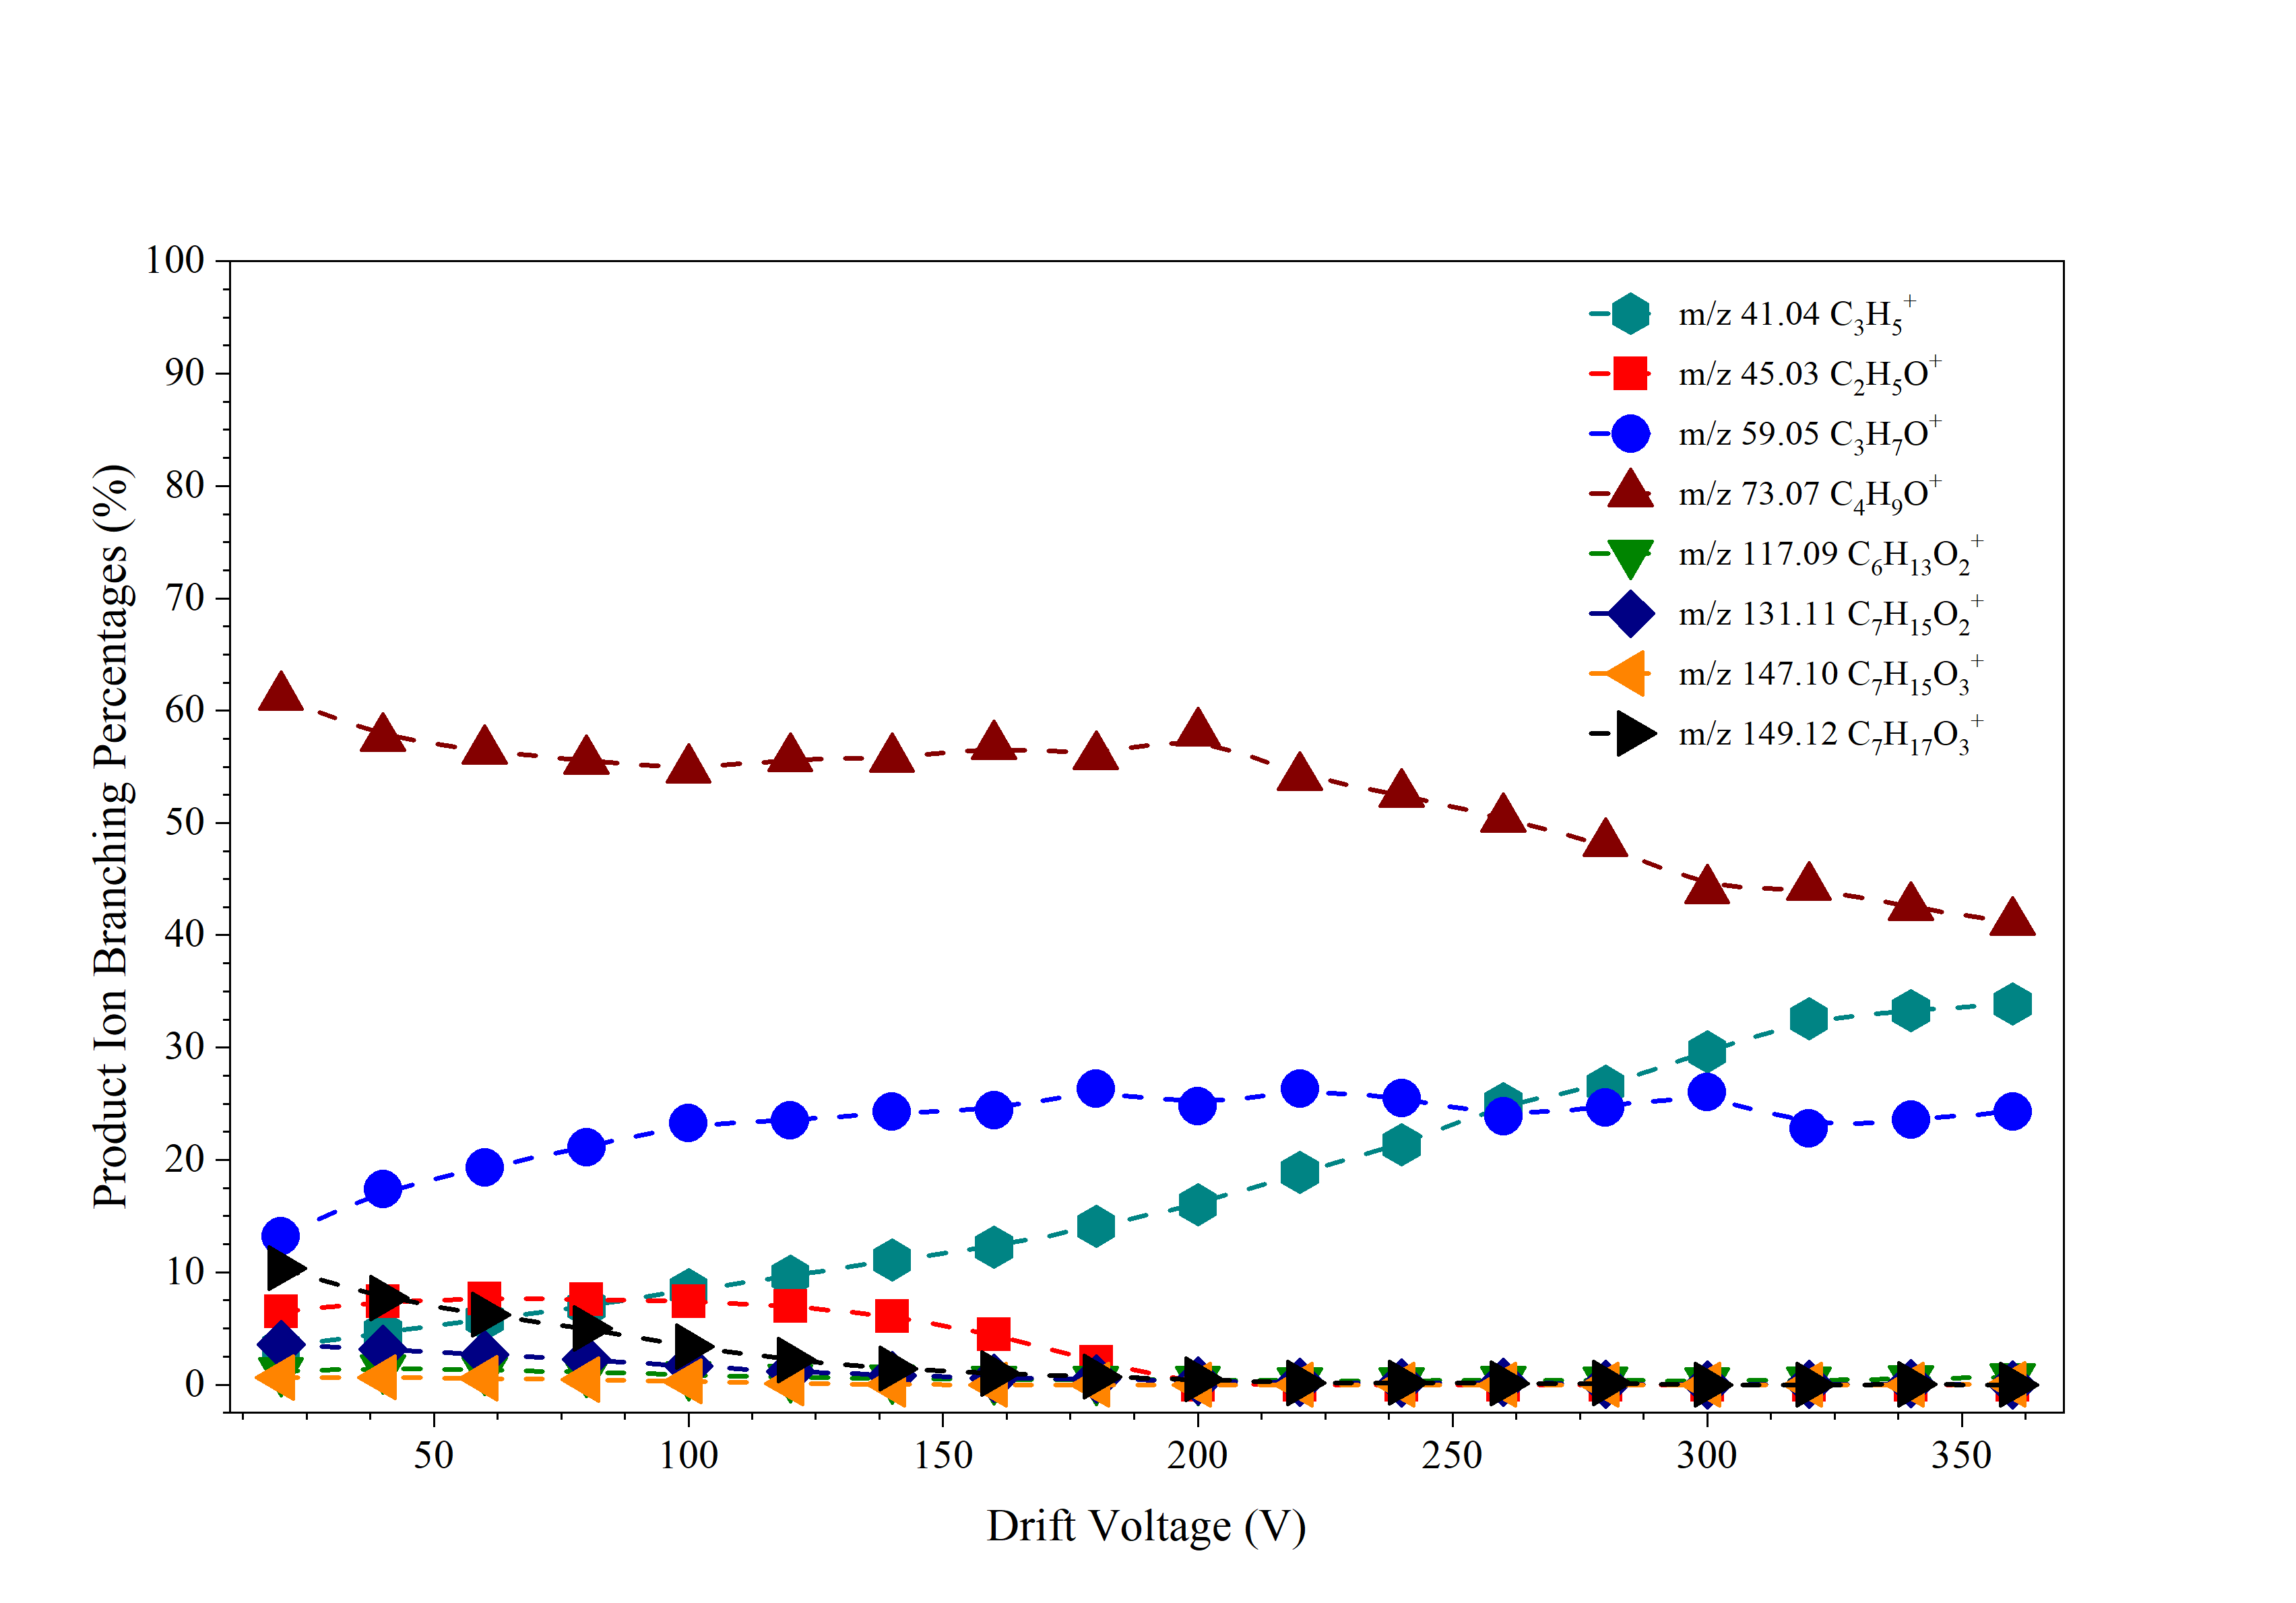
\includegraphics[width=0.48\linewidth]{pics/DPM_humid_RF.png}

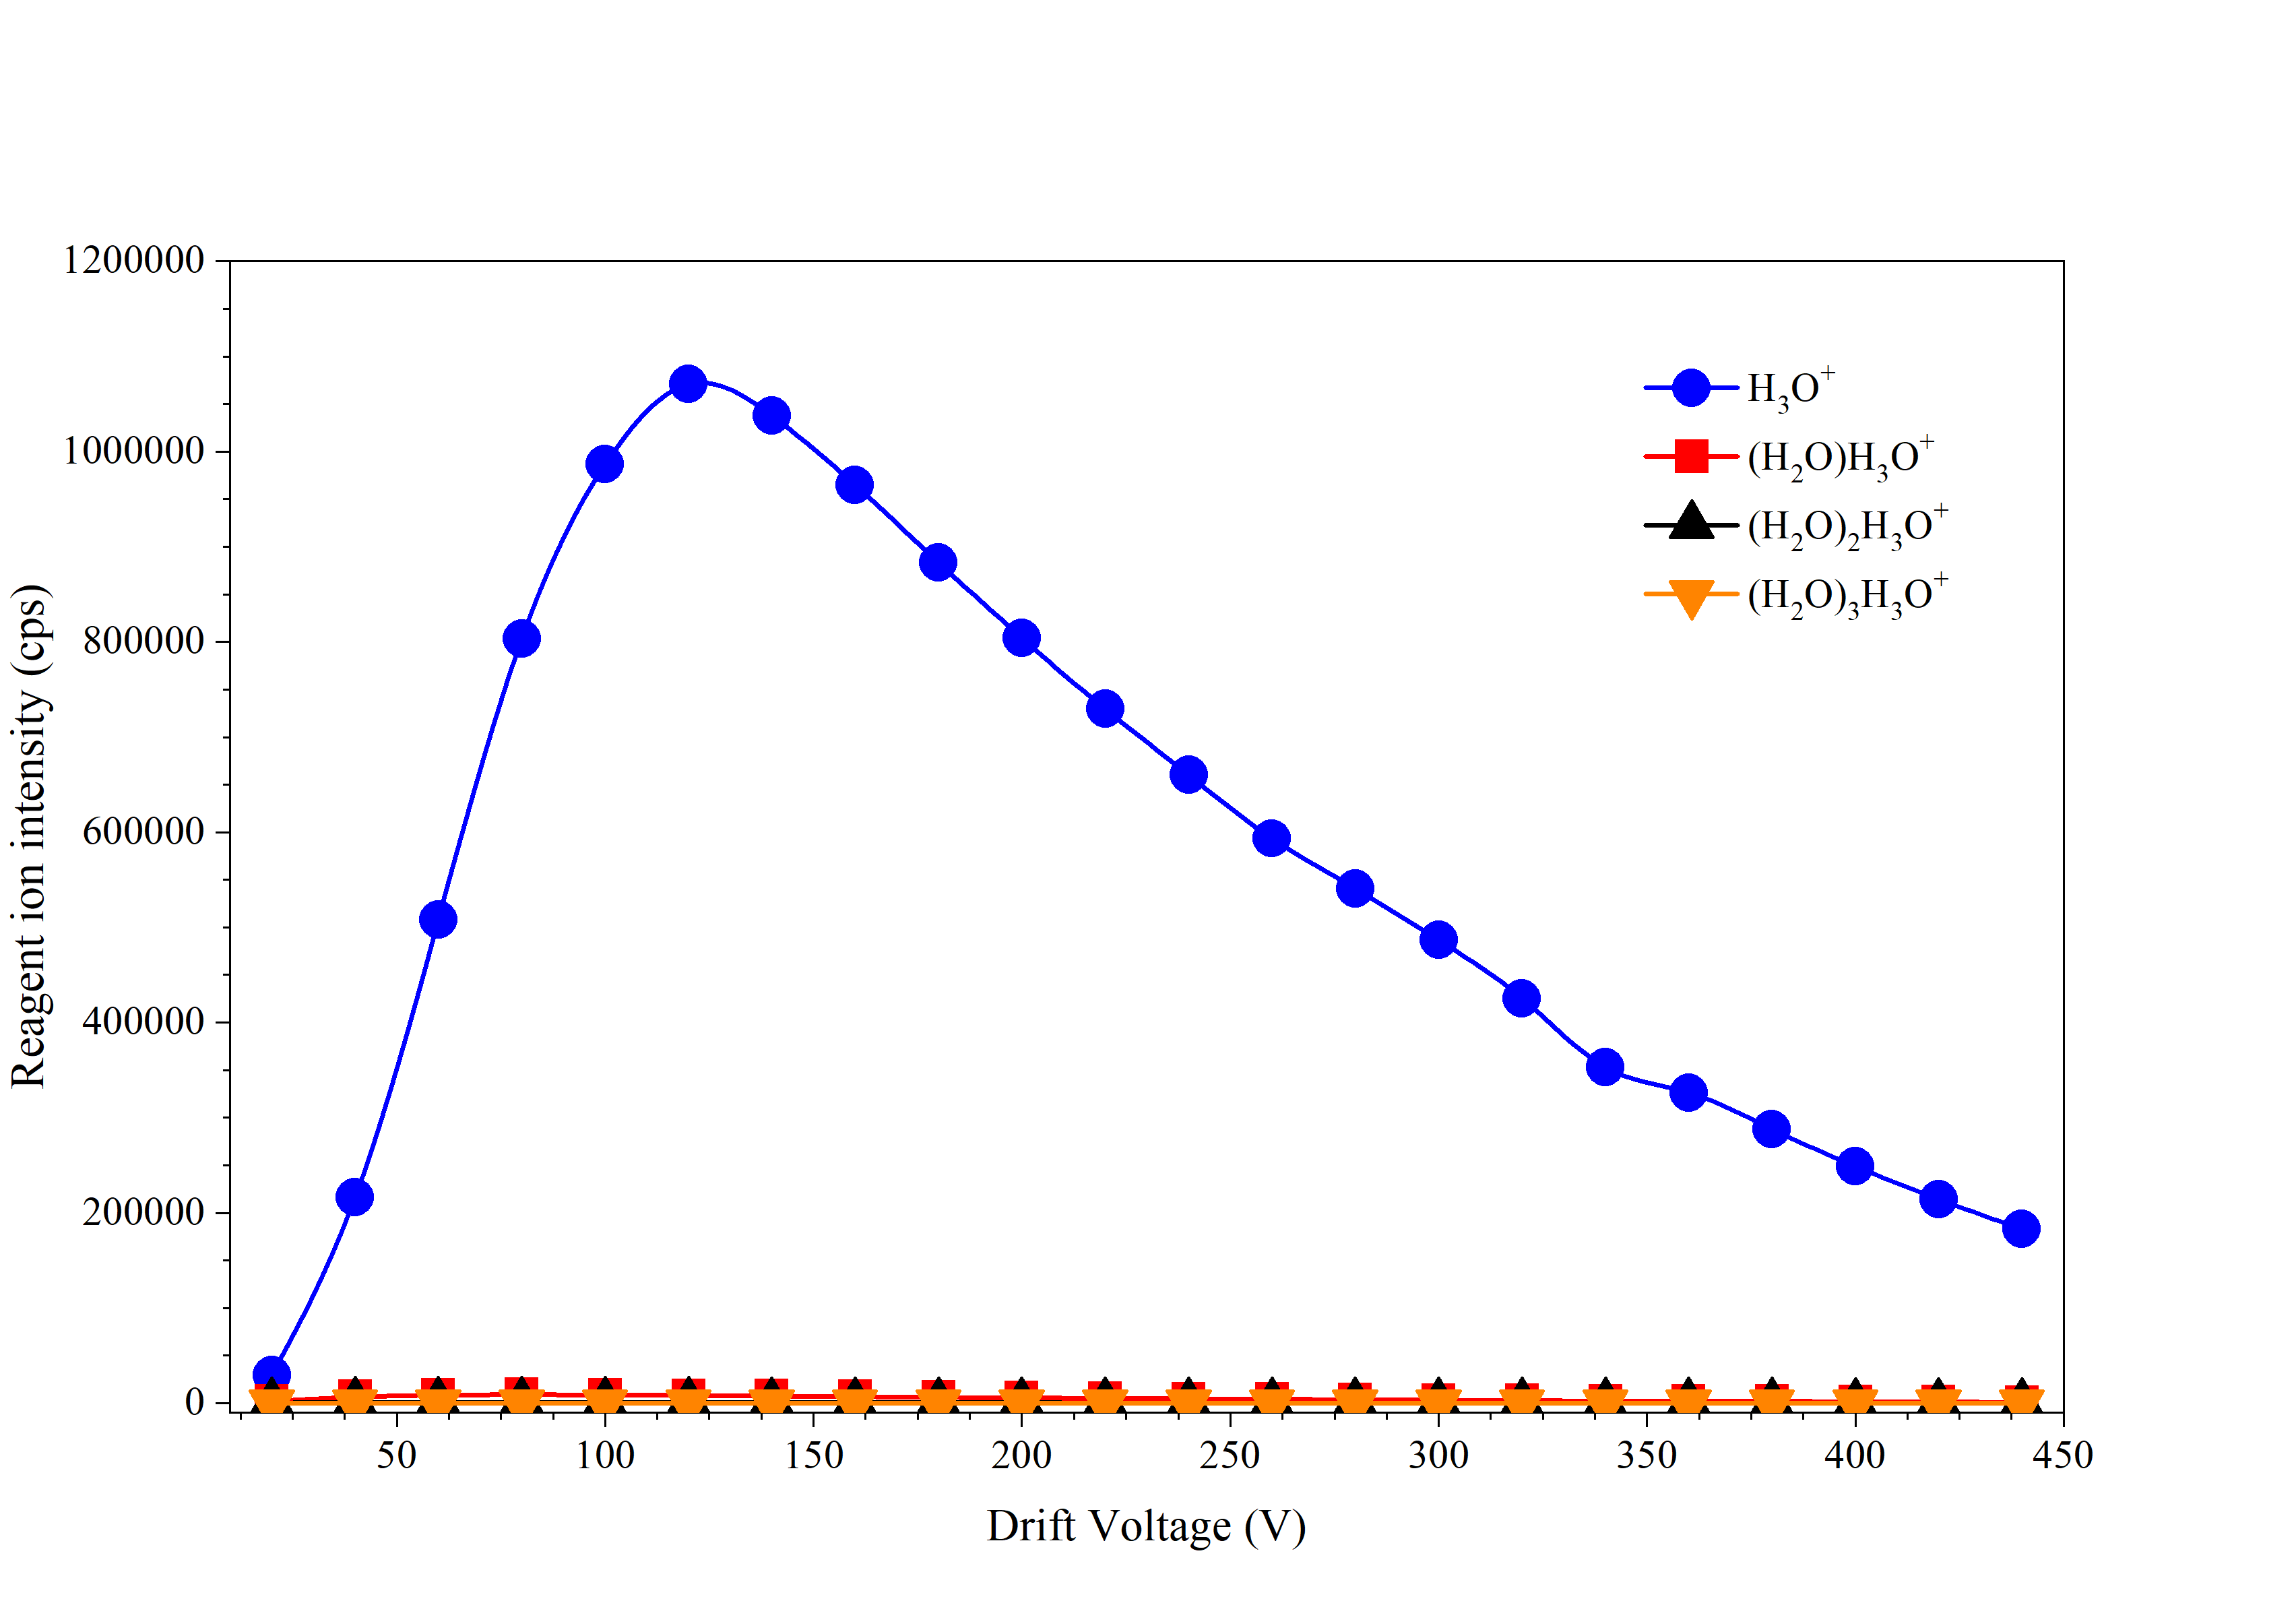
\includegraphics[width=0.48\linewidth]{pics/DPM_clusters_dry_RF.png}
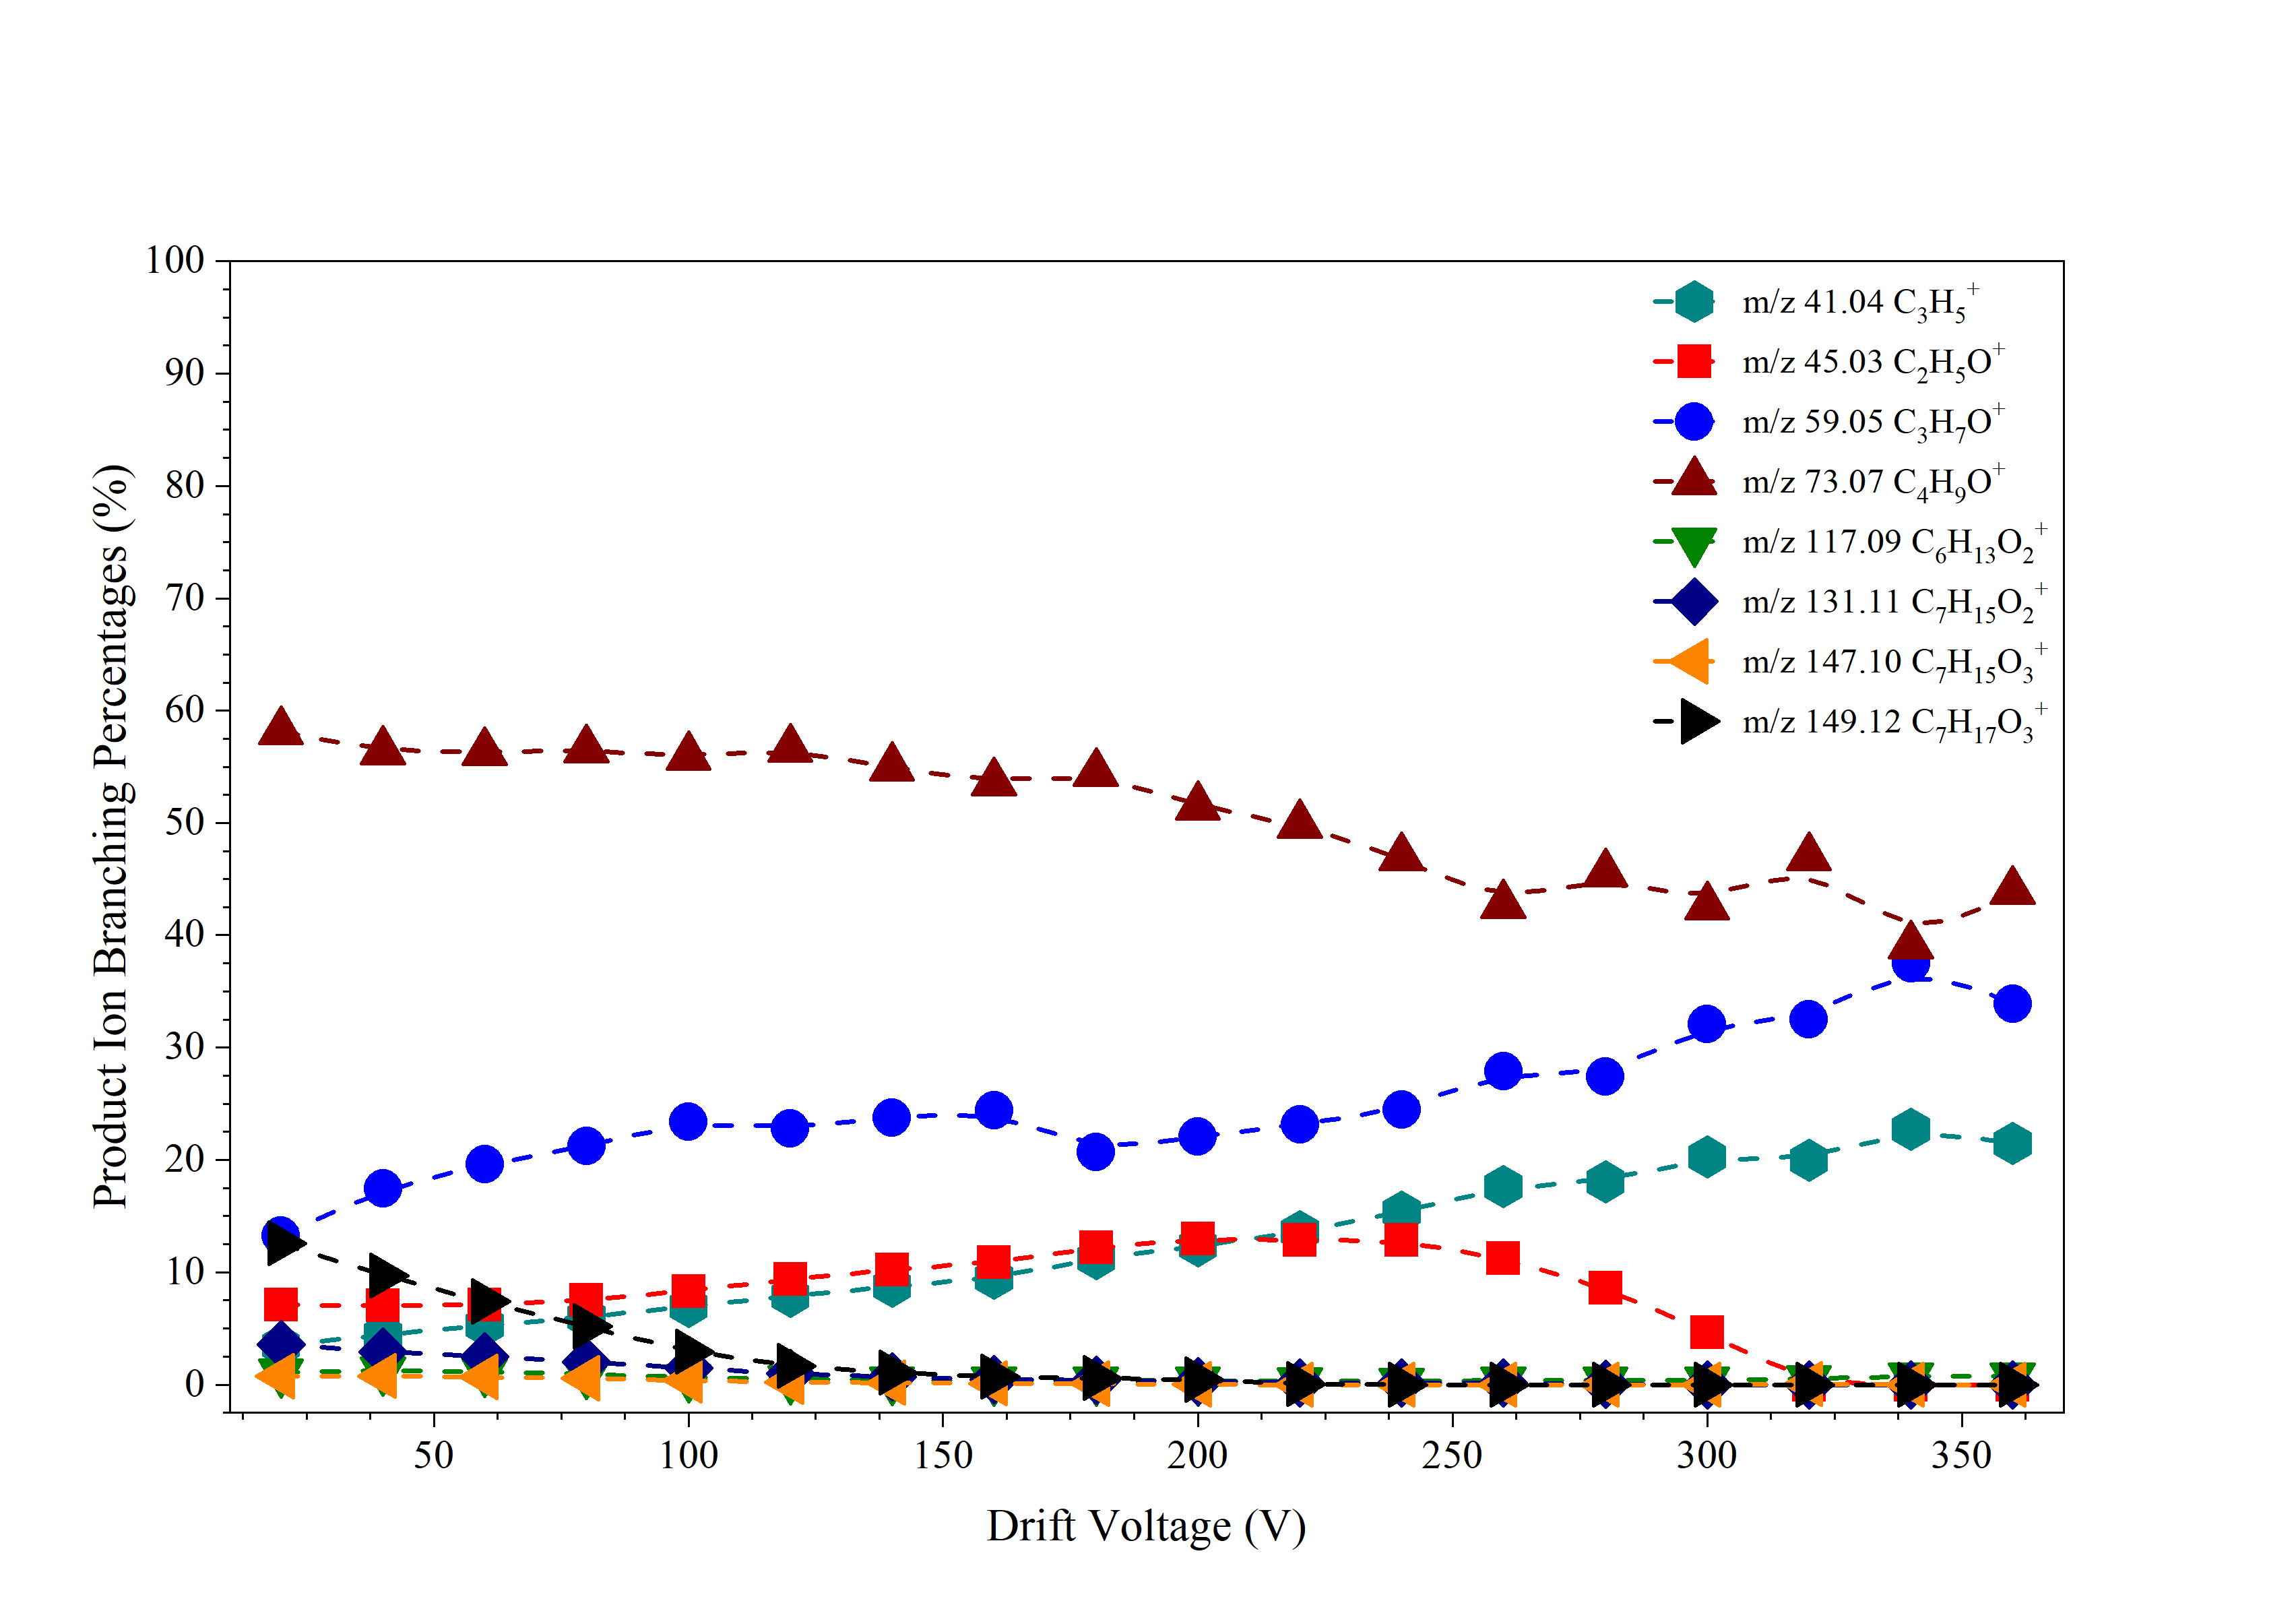
\includegraphics[width=0.48\linewidth]{pics/DPM_dry_RF.png}
\caption{DPM product ion distribution plots from Lynx in humid (top) and  dry (bottom) conditions in RF mode.}
\label{fig:dpm2}
\end{figure}






\section{Dyglyme, etc}
\begin{figure}%[h]
\centering
\vspace{1cm}
\sidesubfloat[]{\scalebox{0.6}{\chemfig{[:30]-[::-60]-[::60]O-[::-60]-[::60]-[::-60]O-[::60]-[::-60]-[::60]O-[::-60]-[::60]}}}\label{fig:dgde1}
\quad
\sidesubfloat[]{\scalebox{0.6}{\chemfig{[:30]-[::-60]O-[::60]-[::-60]-[::60]O-[::-60]-[::60]-[::-60]O-[::60]}}}\label{fig:dgde2}
\vspace{1cm}
\caption{Structure of (a) diethylene glycol diethyl ether and (b) diethylene glycol dimethyl ether}\label{fig:dgde}
\end{figure}






